\documentclass[oneside]{book}
\usepackage[a4paper, total={6in, 8in}]{geometry}
\usepackage[italian]{babel}
\usepackage[utf8]{inputenc}
\usepackage[T1]{fontenc}
\usepackage{listings}
\usepackage{hyperref}
\usepackage{siunitx}
\usepackage{fancyhdr}
\pagestyle{fancy}
\usepackage{textcomp}
\usepackage{makecell}
\usepackage[font=small,labelfont=bf]{caption} 
\usepackage{pdfpages}
\usepackage{multicol}
\usepackage[ruled,vlined]{algorithm2e}

\pagestyle{fancy}
\fancyhf{}
\lhead{\rightmark}
\cfoot{\leftmark}
\rfoot{\thepage}

\lstset{
    frame=tb, % draw a frame at the top and bottom of the code block
    tabsize=4, % tab space width
    showstringspaces=false, % don't mark spaces in strings
    numbers=none, % display line numbers on the left
    commentstyle=\color{green}, % comment color
    keywordstyle=\color{red}, % keyword color
    stringstyle=\color{blue}, % string color
    breaklines=true,
    postbreak=\mbox{\textcolor{green}{$\hookrightarrow$}\space}
}

\renewcommand{\lstlistingname}{}% Listing -> Algorithm
\renewcommand{\lstlistlistingname}{Algoritmi}% List of Listings -> List of Algorithms
\author{
  Giacomo Fantoni \\
  \small Telegram: \href{https://t.me/GiacomoFantoni}{@GiacomoFantoni} \\[3pt]
  Github: \href{https://github.com/giacThePhantom/AlgoritmiStruttureDati}{https://github.com/giacThePhantom/AlgoritmiStruttureDati}}


\renewcommand*{\listalgorithmcfname}{}
\renewcommand*{\algorithmcfname}{}
\renewcommand*{\algorithmautorefname}{}
\renewcommand{\thealgocf}{}


\title{\Huge \textbf{Sistemi operativi}}

\author{
  Giacomo Fantoni \\
  \small Telegram: \href{https://t.me/GiacomoFantoni}{@GiacomoFantoni} \\[3pt]
  Filippo Momesso \\
  \small Telegram: \href{https://t.me/Momofil31}{@Momofil31} \\[3pt]
  \small Github: \href{https://github.com/giacThePhantom/SistemiOperativi}{https://github.com/giacThePhantom/SistemiOperativi}}
\begin{document}
\maketitle
\tableofcontents

\chapter{Introduzione}
Un sistema operativo è un insieme di programmi che agiscono come intermediario tra l'hardware e l'uomo per facilitare l'uso del computer, rendere efficiente l'uso dell'hardware e evitare conflitti
nell'allocazione di risorse tra hardware e software. Offre pertanto un ambiente per controllare e coordinare l'utilizzo dell'hardware da parte dei programmi applicativi. I suoi compiti principali sono di gestore di
risorse e di controllore dell'esecuzione dei programmi e il corretto utilizzo del sistema. La struttura dei sistemi operativi \`e soggetta a notevole variabilit\`a ad \`e adattabile a criteri di organizzazione estremamente differenti.
\`E pertanto un programma sempre in esecuzione sul calcolatore che generalmente viene chiamato kernel al quale si aggiungono programmi di sistema e programmi applicativi.
\begin{figure}[h]
	\includegraphics[width=\textwidth]{Pictures/StackSistemaOperativo.png}
	\caption{Stack del sistema operativo}
\end{figure}
Nel progettare un sistema operativo si deve tipicamente fare un trade-off tra l'astrazione che semplifica l'utilizzo del sistema e l'efficienza.
\subsubsection{Componenti}
Un sistema di calcolo si pu\`o dividere in $4$ componenti:
\begin{itemize}
	\item Dispositivi fisici: sono composti dall'unit\`a centrale di elaborazione (CPU), dalla memoria e dall'I/O.
	\item Programmi applicativi: definiscono il modo in cui utilizzare le risorse per risolvere i problemi computazionali da parte degli utenti.
	\item Sistema operativo: Controlla e coordina l'uso dei dispositivi da parte degli utenti.
	\item Utenti.
\end{itemize}
\subsection{Punti chiave nel progetto di calcolatori}
\subsubsection{Punto di vista dell'utente}
La percezione di un calcolatore dipende dall'interfaccia impiegata. Il pi\`u comune metodo di utilizzo \`e il PC composto da schermo, tastiera e mouse. Il sistema operativo in questo caso si progetta considerando la facilit\`a di
utilizzo con qualche attenzione alle prestazioni ma non all'utilizzo delle risorse. Nel caso di un utente che utilizza terminali connessi ad un mainframe condividendo risorse con altri utenti il sistema operativo andrebbe ottimizzato
per massimizzare l'utilizzo delle risore.
\subsubsection{Punto di vista del sistema}
Il sistema operativo \`e il programma collegato pi\`u strettamente ai suoi elementi fisici ed \`e assimilabile ad un assegnatore di risorse o come programma di controllo che gestisce l'esecuzione dei programmi utente in modo da
impedire che si verifichino errori o che il calcolatore sia utilizzato in modo scorretto.
\section{Storia dei sistemi operativi}
Si possono identificare 5 generazioni di calcolatori che riflettono direttamente l'evoluzione dei sistemi operativi dovuta all'aumento dell'utilizzo del processore.
\subsection{Prima generazione (1946-1955)}
In questa generazione i calcolatori erano enormi e a valvole, non esisteva il sistema operativo e l'operatore del calcolatore era equivalente al programmatore. L'accesso alla macchina era gestito tramite
prenotazioni e i programmi venivano eseguiti da console caricando in memoria un'istruzione alla volta agendo su interruttori. Il controllo degli errori era fatto attraverso spie della console. Il processing era
seriale.
\subsubsection{Evoluzione}
Durante la prima generazione si diffondono periferiche come il lettore/perforatore di schede, nastri e stampanti che rendono necessari programmi di interazione con periferiche detti device driver. Viene
sviluppato del software come librerie di funzioni comuni e compilatori, linker e loader. Queste evoluzioni portano a una scarsa efficienza in quanto pur essendo la programmazione facilitata le operazioni erano
complesse con tempi di setup elevati e un basso utilizzo relativo della CPU per eseguire il programma.
\subsection{Seconda generazione (1955-1965)}
In questa generazione si introducono i transistor nei calcolatori. Viene separato il ruolo di programmatore e operatore eliminando lo schema  a prenotazione e il secondo permette di eliminare dei tempi morti.
I programmi o jobs simili nell'esecuzione vengono raggruppati in batch in modo da aumentare l'efficienza ma aumentando i problemi in caso di errori o malfunzionamenti.
\subsubsection{Evoluzione}
Nasce l'automatic job sequencing in cui il sistema si occupa di passare da un job all'altro: il sistema operativo fa il lavoro dell'operatore e rimuove i tempi morti. Nasce pertanto il monitor residente, il primo
esempio di sistema operativo, perennemente caricato in memoria. Le componenti del monitor erano i driver per i dispositivi di I/O, il sequenzializzatore dei job e l'interprete delle schede di controllo (per la loro
lettura ed esecuzione). La sequenzializzazione avviene tramite un linguaggio di controllo o job control language attraverso schede o record di controllo.
\subsubsection{Limitazioni}
L'utilizzo del sistema risulta ancora basso a causa del divario di velocit\`a tra I/O e CPU. Una soluzione \`e la sovrapposizione delle operazioni di I/O e di elaborazione. Nasce cos\`i l'elaborazione off-line grazie
alla diffusione di nastri magnetici capienti e veloci. La sovrapposizione avviene su macchine diverse: da scheda a nastro su una macchina e da nastro a CPU su un'altra. La CPU viene limitata ora dalla velocit\`a dei
nastri, maggiore di quella delle schede.
\subsubsection{Sovrapposizione tra CPU e I/O}
\`E possibile attraverso un opportuno supporto strutturale far risiedere sulla macchina le operazioni off-line di I/O e CPU.
\paragraph{Polling}
Il polling \`e il meccanismo tradizionale di interazione tra CPU e I/O: avviene l'interrogazione continua del dispositivo tramite esplicite istruzioni bloccanti. Per sovrapporre CPU e I/O \`e necessario un
meccanismo asincrono o richiesta  I/O non bloccante come le interruzioni o interrupt e il DMA (direct memory access).
\paragraph{Interrupt e I/O}
In questo caso la CPU programma il dispositivo e contemporaneamente il dispositivo controllore esegue. La CPU, se possibile prosegue l'elaborazione. Il dispositivo segnala la fine dell'elaborazione alla CPU. La
CPU riceve un segnale di interrupt esplicito e interrompe l'istruzione corrente salvando lo stato, salta a una locazione predefinita, serve l'interruzione trasferendo i dati e riprende l'istruzione interrotta.
\paragraph{DMA e I/O}
Nel caso di dispositivi veloci gli interrupt sono molto frequenti e porterebbero a inefficienza. Si rende pertanto necessario creare uno specifico controllore hardware detto DMA controller che si occupa del
trasferimento di blocchi di dati tra I/O e memoria senza interessare la CPU. Avviene pertanto un solo interrupt per blocco di dati.
\paragraph{Buffering}
Si dice buffering la sovrapposizione di CPU e I/O dello stesso job. Il dispositivo di I/O legge o scrive pi\`u dati di quanti richiesti e risulta utile quando la velocit\`a dell'I/O e della CPU sono simili. Nella realt\`a i
dispositivi di I/O sono pi\`u lenti della CPU e pertanto il miglioramento \`e marginale.
\paragraph{Spooling}
Si dice spooling (simultaneous peripheral operations on-line) )la sovrapposizione di CPU e I/O di job diversi, Nasce un problema in quanto i nastri magnetici sono sequenziali e pertanto il lettore di schede non
pu\`o scrivere su un'estremit\`a del nastro mentre la CPU legge dall'altra. Si devono pertanto introdurre dischi magnetici ad accesso causale. Il disco viene utilizzato come un buffer unico per tutti i job. Nasce
il paradigma moderno di programma su disco che viene caricato in memoria, la pool di job e il concetto di job scheduling (la decisione di chi deve o pu\`o essere caricato su disco).
\subsection{Terza generazione (1965-1980)}
In questa generazione viene introdotta la multiprogrammazione e i circuiti integrati. La prima nasce dal fatto che un singolo job \`e incapace di tener sufficientemente occupata la CPU e pertanto si rende
necessaria una loro competizione. Sono presenti pi\`u job in memoria e le fasi di attesa vengono sfruttate per l'esecuzione di un nuovo job.
Con la presenza di pi\`u job nel sistema diventa possibile modificare la natura dei sistemi operativi: si passa ad una tendenza a sodisfare molti utenti che
operano interattivamente e diventa importante il tempo di risposta di un job (quanto ci vuole perch\`e inizi la sua esecuzione). Nasce pertanto il
multitasking o time sharing, estensione logica della multiprogrammazione in cui l'utente ha l'impressione di avere la macchina solo per s\`e e si migliora
l'interattivit\`a con la gestione di errori e l'analisi di risultati. Nascono i sistemi moderni con tastiera che permette decisioni dell'evoluzione del
sistema in base ai comandi dell'utente e un monitor che permette un output immediato durante l'esecuzione. Il file system inoltre \`e un'astrazione del
sistema operativo per accedere a dati e programmi.
\subsubsection{Protezione}
Con la condivisione si rende necessario introdurre delle capacit\`a di protezione per il sistema:
\begin{itemize}
	\item I/O: programmi diversi non devono usare il dispositivo contemporaneamente, viene realizzata tramite il modo duale di esecuzione: modo user in cui i
	      job non possono accedere direttamente alle risorse di I/O e modo supervisor o kernel in cui il sistema operativo pu\`o accedere a tali risorse. Tutte le
	      operazioni di I/O sono privilegiate: le istruzioni di accesso invocano una system call, un interrupt software che cambia la modalit\`a da user a supervisor
	      e al termine della system call viene ripristinata la modalit\`a utente.
	\item Memoria: un programma non pu\`o leggere o scrivere ad una zona di memoria che non gli appartiene: realizzata associando dei registri limite ad ogni
	      processo, che possono essere modificati unicamente dal sistema operativo con istruzioni privilegiate.
	\item CPU: prima o poi il controllo della CPU deve tornare al sistema operativo, realizzata attraverso un timer legato ad un job, al termine del quale il
	      controllo passa al monitor.
\end{itemize}
\subsection{Quarta generazione (1980-1990)}
\begin{itemize}
	\item Diffusione di sistemi operativi per PC e workstation, utilizzo personale degli elaboratori e nascita delle interfacce grafiche (GUI).
	\item Sistemi operativi di rete in cui esiste una separazione logica delle risorse remote in cui l'accesso alle risorse remote \`e diverso rispetto a quello
	      delle risorse locali.
	\item Sistemi operativi distribuiti: le risorse remote non sono separate logicamente e l'accesso alle risorse remote e locali \`e uguale.
\end{itemize}
\subsubsection{Quinta generazione (1990- oggi)}
Sistemi real-time vincolati sui tempi di risposta del sistema, sistemi operativi embedded per applicazioni specifiche, per piattaforme mobili e per
l'internet of things.

\chapter{Componenti di un sistema operativo}
Un sistema operativo offre un ambiente in cui eseguire i programmi e fornire servizi che naturalmente variano in base al sistema operativo. Si possono comunque identificare alcune classi di servizi comuni.
\section{Servizi di gestione}
\subsubsection{Gestione dei processi}
Si intende per processo un programma in esecuzione che necessita di risorse e viene eseguito in modo sequenziale (un'istruzione alla volta). Si differenzia tra processi del sistema operativo e quelli utente. Il 
sistema operativo \`e responsabile della creazione, distruzione, sospensione, riesumazione e della fornitura di meccanismi per la sincronizzazione e la comunicazione tra processi.
\subsubsection{Gestione della memoria primaria}
La memoria primaria conserva dati condivisi dalla CPU e dai dispositivi di I/O. Un programma deve essere caricato in memoria prima di poter essere eseguito. Il sistema operativo \`e responsabile della gestione 
dello spazio di memoria (quali parti e da chi sono usate), ovvero della decisione su quale processo caricare in memoria in base allo spazio disponibile e dell'allocazione e rilascio dello spazio di memoria. 
\subsubsection{Gestione della memoria secondaria}
Essendo la memoria primaria volatile e piccola si rende necessaria una memoria secondaria per mantenere grandi quantit\`a di dati in modo permanente. \`E formata tipicamente da un insieme di dischi 
magnetici (che stanno per essere sostituiti dai dischi a stato solido -SSD- pi\`u veloci e performanti). Il sistema operativo \`e responsabile della gestione dello spazio libero su disco, dell'allocazione dello spazio su disco e 
dello scheduling degli accessi su disco. 
\subsubsection{Gestionde dell'I/O}
Il sistema operativo nasconde all'utente le specifiche caratteristiche dei dispositivi di I/O per motivi di efficienza e protezione. Viene impegato un sistema per accumulare gli accessi ai dispositivi (buffering), una generica 
interfaccia verso i device driver, con device driver specifici per alcuni dispositivi. 
\subsubsection{Gestione dei file}
Le informazioni sono memorizzate su supporti fisici diversi controllati da driver con caratteristiche diverse. Si crea pertanto un file, un'astrazione logica per rendere conveniente l'uso di memoria non volatile 
grazie alla raccolta di informazioni correlate. Il sistema operativo \`e responsabile della creazione e cancellazione di file e directory, del supporto di operazioni primitive per la loro gestione (copia, incolla, modifica), 
della corrispondenza tra file e spazio fisico su disco e del salvataggio delle informazioni a scopo di backup. 
\subsubsection{Protezione}
Si intende con protezione un meccanismo per controllare l'accesso alle risorse da parte di utenti e processi. Il sistema operativo deve definire quali sono gli accessi autorizzati e quali no, i controlli da imporre e fornire gli 
strumenti per verificare le politiche di accesso. La sicurezza di un sistema operativo comincia con l'obbligo di identificazione di ciascun utente che permette l'accesso alle risorse.  
\subsubsection{Rete (sistemi distribuiti)}
Si intende per sistema distribuito una collezione di elementi di calcolo che non condividono n\`e la memoria n\`e un clock: le risorse di calcolo vengono connesse tramite una rete. Il sistema operativo \`e 
responsabile della gestione in rete delle varie componenti.
\section{Interprete dei comandi (shell)}
Vi sono due modi fondamentali per gli utenti di comunicare con il sistema operativo: un primo basato su un'interfaccia a riga di comando (o interprete dei comandi) e un secondo bastato su un'interfaccia grafica o GUI. Il primo lascia
inserire direttamente agli utenti le istruzioni che il sistema deve eseguire. L'interprete dei comandi \`e pi\`u comunemente conosciuto come shell. La funzione principale dell'interprete \`e quella di prelevare ed eseguire il successivo
comando impartito dall'utente. A questo livello si usano nuovi comandi per la gestione dei file che possono essere implementati internamente all'interprete o attraverso programmi speciali. Nel secondo caso l'interprete non capisce il
comando in s\`e ma prende il nome per caricare l'opportuno file in memoria per eseguirlo.
\subsubsection{Interfaccia grafica}
L'interfaccia grafica \`e una modalit\`a di comunicazione tra utente e il sistema operativo. \`E pi\`u intuitiva della riga di comando e la GUI \`e l'equivalente del desktop e rimane strettamente legata a mouse, tastiera e schermo.
Puntando le icone col mouse \`e possibile accedere a file, cartelle e applicazioni. 
\subsection{System calls}
Le chiamate di sistema costituiscono l'interfaccia di comunicazione tra il processo e il sistema operativo. Sono tipicamente scritte in linguaggi di alto livello come \emph{C} o \emph{C++}. I programmatori non si devono preoccupare dei
dettagli di implementazione delle \emph{sys.call} in quanto solitamente utilizzano un'API (application program interface) che specifica un'insieme di funzioni a disposizione dei programmatori e dettaglia i parametri necessari 
all'invocazione di queste funzioni e i valori restituiti. Le due API pi\`u comuni sono \emph{win32} e \emph{POSIX API}, rispettivamente per Windows e UNIX. I parametri delle system calls possono essere pasati per valore o riferimento, ma
vanno fisicamente messi da qualche parte: vengono pertanto posizionati nei registri (molto veloci, ma pochi e di dimensione fissa) nello stack del programma o in una tabella di memoria il cui indirizzo \`e passato in un registro o nello
stack. Le system calls possono essere implementate in due modi: 
\begin{itemize}
	\item L'interprete legge il comando e cerca all'interno della shell per cercare il programma da avviare, non viene utilizzata in quanto rende necessario modifiche al kernel e non
		\`e efficiente.
	\item L'interprete legge il comando e possiede una tabella che collega tale comando al programma da avviare. 
\end{itemize}
Le system calls si differiscono in controllo dei processi, gestione dei file, dei dispositivi, delle comunicazioni e della protezione. Un processo inoltre 
deve essere sia in grado di essere chiuso normalmente (\emph{end}) che in modo anomalo (\emph{abort}), con la conseguente generazione di un messaggio di 
errore e copia dello stato del processo abortito.

\chapter{Architettura di un sistema operativo}
Un principio importante \`e la separazione tra meccanismi e criteri o policy: i primi determinano come eseguire qualcosa, mentre i secondi cosa si deve fare. Questa distinzione \`e importante ai fini della
flessibilit\`a in quanto i criteri sono soggetti a cambiamenti di luogo e tempo. Principi importanti da tenere a mente durante lo sviluppo di sistemi operativi \`e il KISS (keep it small
and simple), semplice dal punto di vista del codice, per mantenere affidabilit\`a e mantenibilit\`a e il POLA (principle of least privilege): un programma deve poter accedere unicamente ai
dati strettamente necessari, fondamentale per il mantenimento di sicurezza e affidabilit\`a. Questi cambiamenti devono richiedere il cambio di meccanismi solo nel caso pessimo. Le 
principali tipologie di architettura di sistemi operativi sono:
\begin{itemize}
	\item Sistemi monolitici: sistemi senza gerarchia e con un unico strato software tra utente e hardware, tutti i componenti sono sullo stesso 
		livello e possono chiamarsi vicendevolmente. In questa tipologia il codice dipende direttamente dall'architettura hardware e rende test
		e debugging complesso.
	\item Sistemi a struttura semplice: si ha un minimo di gerarchia e di struttura, non esiste  ancora la suddivisione modalità utente e modalità kernel. Questa struttura \`e mirata a ridurre i costi di sviluppo e manutenzione.
	\item Sistema operativo a livelli. I servizi sono organizzati su livello gerarchici con al livello pi\`u alto l'interfaccia utente e al pi\`u 
		basso l'hardware. Ogni livello pu\`o utilizzare funzioni di livelli inferiori. La modularit\`a rende pi\`u semplice la manutenzione, ma
		diminuisce l'efficienza e richiede un'attenta definizione dei livelli. 
	\item Sistemi basati su kernel: vengono utilizzati due livelli, i cui servizi sono distinti tra kernel e non-kernel. Presenta i vantaggi del sistema a livelli come modularit\`a
		ma senza avere troppi livelli. Tra i servizi al di fuori del kernel non si trova nessuna organizzazione e si tende a pensare al kernel come a una struttura monolitica.
	\item Sistemi a micro-kernel: i micro-kernel sono un insieme di piccoli kernel che svolgono poche funzioni fondamentali. Occupano meno memoria e sono pi\`u affidabili e 
		mantenibili, ma presentano scarse prestazioni: ogni volta che si deve accedere ad un programma applicativo si deve fare un cambio da modalit\`a kernel a modalit\`a
		utente e viceversa una volta terminato il processo. Vengono utilizzati da quando le prestazioni di CPU e memoria sono sufficienti a non far percepire all'utente il cambio
		di modalit\`a. La modularit\`a offre inoltre maggiore sicurezza e portabilit\`a.
\end{itemize}
\section{Modello client-server}
Una variazione del'idea del microkernel \`e quella di distinguere due classi di processi: i server che forniscono un servizio e i client che lo utilizzano. Spesso il livello pi\`u basso
\`e un microkernel, ma non \`e richiesto. La comunicazione tra client e server avviene tramite scambio di messaggi: per ottenere un servizio il client deve costruire un messaggio e 
inviarlo al server, che quando lo riceve restituisce la risposta. Se client e server operano sulla stessa macchina sono possibili delle ottimizzazioni.  
\section{macchine virtuali}
Le macchine virtuali sono introdotte nel $1972$ da IBM come estremizzazione dell'approccio a livelli pensata per offrire un sistema di timesharing multiplo ovvero che permette la
multiprogrammazione e una macchina estesa che abbia un'interfaccia pi\`u semplice del solo hardware. La base della macchina virtuale \`e la separazione di questi due aspetti. La sua parte
centrale era il virtual machine monitor che permette la multiprogrammazione offrendo diverse macchine virtuali al livello superiore. Un tipo di macchina virtuale utilizza un type 1 
hypervisor, usato comunemente che si trova sull'hardware e permette di eseguire diversi sistemi operativi sulla stessa macchina. Il type 2 hypervisor viene utilizzato su un sistema 
operativo host nel quale l'hypervisor installa il sistema operativo guest in un disco virtuale che il sistema host vede come un file di grandi dimensioni. La differenza tra i due tipi
di hypervisor sta nel fatto che quello di tipo 1 si trova direttamente sull'hardware, mentre il tipo 2 viene creato in un sistema operativo host.
\subsection{Esokernel}
Piuttosto che clonare la macchina, un'altra strategia per ottenere un sottinsieme delle risorse \`e partizionarla. Al livello pi\`u basso si trova un programma eseguito in modalit\`a
kernel che alloca risorse alle virtual machine e controlla le loro prove di utilizzarle. Il vantaggio dell'esokernel \`e che evita un livello di mappatura: in altri metodi \`e necessaria
una mappatura dal disco virtuale a quello fisico, come per tutte le altre risorse. 

\section{Processi e thread}
Attributi (Process Control Block): contiene un puntatore alla cella di memoria che contiene l’immagine, contiene lo stato del processo in un determinato momento, contiene i registri, le informazioni relative allo stato dell’I/O. 
Un processo può essere in diversi stati. 
All’inizio il processo viene creato, poi può essere in esecuzione se gli viene assegnata la CPU o non in esecuzione se non gli viene assegnata la CPU. Il Dispatcher assegna la CPU ai processi che sono pronti, ma non in esecuzione (posso 
avere diversi processi in memoria, ma solo uno per volta usa la CPU e quindi è effettivamente in esecuzione, a meno di CPU multicore). Quando un processo è pronto e viene creato viene messo nella ReadyQueue (oppure nella coda di un 
dispositivo cioè la coda in cui viene messo un processo che sta aspettando di accedere a un determinato dispositivo). In realtà esistono diverse code in cui può essere messo un processo. Dispatch e Scheduler sono due componenti diversi, 
lo scheduler sceglie mentre il dispatcher implementa questa cosa. Context-Switch: salvo tutto quello che c’era nel PCB, tutto quello che stavo utilizzando al momento dell’esecuzione. Due operazioni fondamentali che fa un sistema operativo
è la creazione e la terminazione del processo. Ogni processo può creare altri processi e questi prendono il nome di processi figli. Il figlio può essere creato in modalità sincrona, cioè finché il figlio è in vita io non faccio niente, 
oppure in modalità asincrona cioè io creo il figlio e continuo la mia esecuzione. Con la fork il figlio lo creo esattamente uguale al padre, con la exec posso caricare sul figlio un programma diverso rispetto al padre. Con la wait creo 
un’esecuzione sincrona tra padre e figlio. Una fork può fallire perché o il padre non ha abbastanza memoria o perché non ha i privilegi per creare un figlio. L’exec cambia l’immagine in memoria del figlio.

\chapter{Processi e threads}
Il concetto centrale per ogni sistema operativo \'e quello di processo, l'astrazione di un programma che sta venendo eseguito. Tali astrazioni permettono
di avere operazioni pseudo-concorrenti anche quando esiste una sola CPU, trasformandola in diverse CPU virtuali.
\section{Processi}
Tutti i computer moderni svolgono diverse funzioni allo stesso tempo. In un sistema multiprogramma la CPU cambia da processo a processo rapidamente,
eseguendo ognuno per decine o centinaia di millisecondi. Si parla di pseudoparallelismo in contrasto con il parallelismo dei sistemi multiprocessore. .
\subsection{Il modello dei processi}
In questo modello tutti il software eseguibile sul computer \`e organizzato in un numero di processi sequenziali, istanze di un programma che sta venendo eseguito con i valori per
il contatore, i registri e le variabili. Ogni processo possiede la propria CPU virtuale, anche se \`e la CPU che cambia tra i processi, chiamato multiprogramming. Ogni programma in
questo caso viene eseguito in maniera indipendente. Essendo che esiste un unico contatore di programma fisico, quando un processo viene eseguito il suo contatore logico \`e inserito
in quello reale. Quando si passa ad un altro processo il contatore fisico \`e salvato nel contatore logico del processo. Si assuma che ci sia una sola CPU. Con essa che cambia tra i
processi, il tasso di computazione di un processo non sar\`a uniforme n\`e riproducibile, pertanto i processi non possono essere programmati con assunzioni riguardo alla temporizzaizone.
Quando un processo richiede dei criteri real-time eventi si devono prendere delle misure speciali. Il processo pu\`o essere considerato come un'istanza del programma, con un input, un
output e uno stato. Si noti come se un programma viene eseguito due volte conta come due proessi.
\subsection{Creazione dei processi}
I sistemi operativi necessitano di un modo per creare processi. In sistemi progettati per eseguire una singola applicazione potrebbe essere possibile avere tutti i processi che saranno
necessari presenti allo startup. In sistemi general-purpose \`e neccessario avere qualche modo per creare e terminare processi quando sono necessari durante l'operazione. Ci sono
quattro princupali cause per la creazione di un processo:
\begin{itemize}
	\item Inizializzazione del sistema. Durante la fase di boot sono creati numerosi processi, alcuni che interagiscono con l'utente e altri di background che non sono associati con
	      utenti particolari ma hanno funzioni specifiche. I processi che stanno nel background per gestire delle attivit\`a sono detti daemons e sistemi grossi ne possiedono a
	      dozzine.
	\item Esecuzione di una system call da un processo che sta venendo eseguito che crea un processo attraverso una system call. Creare un nuovo processo \`e utile quando il lavoro
	      che deve essere eseguito pu\`o essere formulato come un insieme di processi che interagiscono ma sono indipendenti.
	\item L'utente richiede di creare il processo in sistemi interattivi attraverso un comando o cliccando su un'icona. In sistemi basati su UNIX il nuovo processo rileva la finestra
	      da dove \`e eseguito. In windows il processo pu\`o creare una o pi\`u finestre. In entrambi i casi l'utente pu\`o avere pi\`u finestre aperte contempoaneamente.
	\item Inizializzazione di un batch job su sistemi batch che si trovano su grandi mainframes. Gli utenti possono inviare batch jobs al sistema e quando il sistema decide che ha
	      le risorse necessarie per eseguirne un altro crea un nuovo processo e svolge il job successivo nella coda.
\end{itemize}
Tecnicamente in tutti questi casi un nuovo processo \`e creato avendo un processo esistente che esegue una system call che dice al sistema operativo di creare un nuovo processo e indica
direttamente o indirettamente quale programma eseguire in esso. In UNIX esiste un'unica system call per creare un nuovo processo: \emph{fork} che crea un clone esatto del processo
chiamante. Dopo la \emph{fork} i due processi hanno la stessa immagine di memoria, le stesse stringhe ambientali e gli stessi file aperti. Tipicamente il processo figlio esegue
\emph{execve} o una system call simile per cambiare l'immagine di memoria e eveguire un nuovo programma. Quando l'utente inserisce un comando la shell forka il processo figlio che poi
esegue il comando. QUesti due passaggi permettono al figlio di manipolare i propri file descriptors dopo la \emph{fork} ma prima dell'\emph{execve}. In Windows una singola chiamata alla
funzione \emph{CreateProcess} gestisce entrambi i passaggi con $10$ parametri che includono la creazione e il caricamento del programma corretto da eseguire, i parametri di liena di
comando, attributi di sicurezza, bit di controllo e un puntatore alla struttura in cui le informazioni sul processo sono ritornate al chiamante. Dopo che un processo \`e creato
il genitore e il figlio possiedono i propri spazi di indirizzamento distinti. In UNIX quello del figlio \`e inizialmente una copia del genitore ma non \`e condivisa memoria scrivibile.
\subsection{Terminazione di un processo}
Dopo che un processo \`e stato creato e ha svolto il suo lavoro termina in:
\begin{itemize}
	\item Normal exit (volontaria), la maggior parte dei processi termina in questo modo eseguendo una system call in modo da dire al sistema operativo che ha finito.
	      Questa call \`e \emph{exit} in UNIX e \emph{ExitProcess} in Windoes. Programmi screen-oriented supportano la terminazione volontaria.
	\item Error exit (volontaria), avviene quando il processo scopre un errore, lo annuncia ed esce, le applicazioni screen oriented tipicamente creano una dialog box.
	\item Fatal error (involontaria) \`e causata da un bug nel programma, come l'esecuzione di un'istruzione illegale.
	\item Ucciso da un altro processo (involontario) attraverso una system call che dice al sistema operativo di terminarlo in UNIX \`e \emph{kill}, in Windows \`e
	      \emph{TerminateProcess}.
\end{itemize}
In alcuni sistemi quando un processo termina sono uccisi anche tutti i processi che ha creato.
\subsection{Gerarchie di processi}
In alcuni sistemi quando un processo ne crea un altro rimangono associati in certi modi. in UNIX un progesso e tutti i suoi discendenti formano un gruppo di processi. Quando un segnale
viene inviato dalla tastiera viene ricevuto da tutti i membri del gruppo di processi associati alla tastiera. Individualmente ogni processo pu\`o catturare il segnale, ignorarlo o
svolgere un'azione default, che \`e di essere ucciso dal sengale. Un altro esempio di gerarchia \`e dato dal inizializzazione di UNIX successivamente la fase di boot. Un processo
speciale detto \emph{init} \`e presente nella immagine di boot e quando viene eseguito legge un file che dice quanti terminali ci sono. Successivamente forka ad un nuovo processo per
terminale. Questi processi aspettano per un login che se hanno successo esegue una shell per eseguire comandi che potrebbero iniziarne altri e cos\`i via. Pertanto tutti i processi
del sistema si basano su un singolo albero con \emph{init} alla radice. Windows non possiede un concetto di gerarchia dei processi: sono tutti uguali, ma quando un processo \`e generato
il padre possiede un token detto handle che gli permette di controllare il figlio. Questo tolen pu\`o essere passato ad altri process, annullando la gerarchia.
\subsection{Stati dei processi}
Nonostante ogni processo sia un'entit\`a indipendente, con il proprio program counter e stato interno, deve spesso interagire con altri processi, ad esempio accettando come input
l'output di altri. Quando un processo si blocca lo sa in quanto non pu\`o continuare logicamente, tipicamente quando sta aspettando per un input che non \`e disponibile. \`E inoltre
possibile che sia bloccato in quanto il sistema operativo ha deciso di allocare la CPU per un altro processo. Queste due condizioni sono diverse in quanto la prima \`e inerente il
problema, mentre nel secondo caso \`e una tecnicalit\`a del sistema. Ci sono pertanto tre stati che il processo pu\`o avere:
\begin{itemize}
	\item Running: il processo sta utilizzando la CPU.
	\item Ready: eseguibile, stoppato per far eseguire un altro processo. Stato logicamente simile al primo in quanto il processo in entrambi i casi \`e capace di essere eseguito.
	\item Blocked: incapace di essere eseguito fino a che un evento esterno accade. Questo stato \`e differente in quanto il processo non pu\`o essere eseguito anche con la CPU
	      libera.
\end{itemize}
L'unica transizione non possibile \`e duella da ready a blocked. La transizione da running a blocked avviene quando il sistema scopre che un processo non pu\`o contineare al momento.
In alcuni sistemi si pu\`o eseguire una system call come \emph{pause} per entrare in uno stato bloccato, in altri sistemi come UNIX, quando un processo legge da una pipe o da un file
speciale e non si trova input disponibile il processo \`e automaticamente bloccato. La transizione da running a ready e viceversa sono causate dallo scheduler dei processi in modo da
permettere l'eventuale esecuzione di tutti i processi in stato ready. La transizione da blocked a running avviene quando un evento esterno elimina il blocco logico del processo.
Il modello dei processi permette di semplificare gli eventi interni al sistema: alcuni processi eseguono comandi dell'utente, altri sono parte del sistema e gestiscono richieste di
esso. Quando avviene un interrupt il sistema ferma il processo corrente ed esegue l'interrupt che si bloccano quando aspettano che accada qualcos altro. Il livello pi\`u basso del
sistema operativo \`e lo scheduler, con un insieme di programmi al di sopra di esso. Tutti i dettagli della gestione dell'interrupt e di blocco e inizio dei processi sono nascosti e il
resto del sistema operativo \`e stutturato in forma di processo.
\subsection{Implementazione dei processi}
Per implementare il modello dei processi il sistema operativo mantiene una tabella (array di strutture) chiamata la tabella dei processi con un entry per processo contenente
informazioni riguardo lo stato del processo, come il program counter, lo stack pointer, la memoria allocata, lo stato dei file aperti e le informazioni di accounting e scheduling e
ogni altra informazione che deve essere salvata quando il processo viene passato da running a ready o blocked in modo che possa essere fatto ripartire successivamente. In un tipico
sistema la tabella presenta tre colonne con la prima dedicata alla gestione del processo, la seconda alla gestione della memoria e la terza alla gestione dei file. Associato con ogni
classe di I/O si trova una locazione (tipicamente fissa al fondo della memoria) detta interrupt vector che contiene l'indirizzo dell procedura del servizio di interrupt. Quando accade
un interrupt tutti i processi che stanno venendo eseguiti salvano il program coutner, lo stato e dei registri nello stack grazie all'hardware di interrupt e il computer salta
all'indirizzo specificato nell'interrupt vector che fa partire la procedura. Tutti gli interrupt cominciano con il salvataggio dei registri nell'entri del processo corrente, dopo
l'informazione \`e pushata sullo stack dall'interrupt \`e rimossa e il puntatore allo stack \`e settato a puntare ad uno stack temporaneo utilizzato dal gestore dei processi. Il
salvataggio dei registri e il settaggio dello stack pointer devono essere svolti da una piccola routine in assembly, uguale per ogni interrupt. Quando la routine \`e finita chiama una
procedura in $C$ che svolge il resto del lavoro specifico al tipo di interrupt. Quando \`e finito viene chiamato lo scheduler per vedere quale processo deve essere eseguito. Dopo
quello il controllo \`e passato al codice in assembly per ricaricare in memoria i registri e le mappe per il proceso corrente e comincia ad essere eseguito. Dopo ogni interrupt il
processo ritorna precisamente nello stesso stato in cui era prima che accadesse l'interrupt. Riassumendo il processo di interrupt:
\begin{itemize}
	\item L'hardware salva lo stato del processo sullo stack.
	\item L'hardware carica il nuovo program counter dall'interrupt vector.
	\item Una procedura in assembly salva i registri.
	\item Una procedura crea un nuovo stack.
	\item Una servizio di interrupt in C viene eseguito (tipicamente legge e buffera l'input).
	\item Lo scheduler decide il prossimo processo da eseguire.
	\item Una procedura in C ritorna il codice in assmbly.
	\item Una procedura in assembly ricomincia il nuovo processo corrente.
\end{itemize}
\subsection{Modellare la multiprogrammazione}
L'utilizzo della multiprogrammazione permette il miglioramento dell'utilizzo della CPU: se il processo medio computa il $20\%$ del tempo che risiede in memoria, $5$ processi alla volta
dovrebbero rendere la CPU occupata tutti il tempo (irrealisticamente ottimistico). Un modello migliore consiste nel guardare l'utilizzo della CPU in modo probabilistico: suppondendo che
un processo utilizzi una frazione $p$ del suo tempo aspettando per il completamento dell'I/O. Con $n$ processi in memoria alla volta, la probabilit\`a che tutti gli $n$ processi stiano
aspettando per l'I/O \`e $p^n$, pertanto l'utilizzo della CPU \`e $1-p^n$. \`E facile notare come siano richiesti molti processi per rendere efficiente l'utilizzo della CPU. Si devono
naturalmente fare delle assunzioni: tutti i processi sono indipendenti mentre con una singola CPU non si possono avere processi che vengono svolti in contemporanea. Pur non essendo
preciso, questo modello d\`a una buona approssimazione delle prestazioni della CPU.
\section{Threads}
Nei sistemi operativi tradizionali ogni processo possiede uno spazio di indirizzamento e un singolo thread di controllo e nonostante questo \`e desiderabile avere multipli thread di
controllo nello stesso spazio di indirizzamento eseguiti quasi in parallelo, quasi come processi separati.
\subsection{Utilizzo dei thread}
La ragione principale alla base dell'utilizzo dei thread \`e che molte applicazioni possiedono multiple attivit\`a che avvengono insieme. Alcune di queste potrebbero bloccarsi. Una
decomposizione in multipli thread sequenziali semplifica il modello di programmazione. Si nota l'analogia con la neccessit\`a di avere i processi, con l'unica differenza che i thread
permettono a entit\`a parallele di condividere uno spazio di indirizzamento e tutti i dati tra di loro, un'abilit\`a fondamentale per certe applicazioni. Oltre a questo i thread sono
pi\`u leggeri e veloci da creare e distruggere dei processi, propriet\`a utile per un sistema dinamico e rapido. Permettono anche una certa sovrapposizione di attivit\`a non legate alla
CPU. Invine sono utili in sistemi con multiple CPU, dove il parallelismo \`e possibile. Esiste un modello di progetatzione in cui lo stato di computazione deve essere salvato e
ripristinato nella tabella ogni volta che si cambia tra le richieste, simulando i threads e i loro stack, chiamato macchine a stato-finito. I thread rendono pertanto possibile mantenere
l'idea dei processi sequenziali che fanno chiamate bloccanti e ottenere parallelismo:\\
\begin{tabular}{|c|c|}
	\hline
	\textbf{Modello}          & \textbf{Caratteristiche}                             \\
	\hline
	Threads                   & Parallelismo, system calls bloccanti                 \\
	\hline
	Processi a thread singolo & Assenza di parallelismo, system calls bloccanti      \\
	\hline
	Macchine a stato finito   & Parallelismo, system calls non bloccanti, interrupts \\
	\hline
\end{tabular}
\subsection{Il modello dei thread classico}
Il modello dei processi si basa sui concetti indipendenti di raggruppamento delle risorse ed esecuzione: i thread permettono la loro separazione. Si pu\`o considerare un processo come
un modo per raggruppare risorse imparentate insieme: possiede uno spazio di indirizzamento che contiene il programma e i dati e altre risorse come file aperti, processi figli, allarmi
in attesa, gestori di segnali, informazioni di gestione che uniti in esso sono gestiti pi\`u facilmente. Il processo inoltre possiede un thread di esecuzione che possiede un program
counter che traccia quale istruzione eseguire successivamente, registri che contengono le variabili correnti, uno stack con la storia dell'esecuzione con un frame per ogni procedura
senza ritorno. Pertanto se i processi raggruppano risorse i thread sono le entit\`a in programma per esecuzione sulla CPU. I thread permettono un esecuzione multipla sullo stesso
ambiente di processo con grande livello di indipendenza. Il termine multithreading \`e utilizzato per descrivere una situazione in cui sono presenti mutlipli thread, detti processi
leggeri. Quando un processo a muiltithread viene eseguito su un sistema a singola CPU i threads fanno a turno come i processi. Thread diversi in un processo non sono indipendenti come
processi diversi: possiedono lo stesso spazio di archiviazione e pertanto devono condividere le stesse variabili globali e possono accedere e modificare i rispettivi stack, non
necessaria in quanto i thread si generano da un processo generato da un utente e sono creati in modo da cooperare. Si nota come pertanto gli oggetti singoli di un processo sono lo
spazio di archiviazione, le variabili globali, file aperti, processi figli, allarmi in attesa, segnali e loro gestori e informazioni di contabilit\`a, mentre un thread possiede il
program counter, i registri, lo stack e lo stato. Nello stesso modo dei processi possono essere eseguiti, bloccati, pronti o terminati. Ogni stack del thread contiene un frame per
ogni procedura che \`e stata chiamata ma non ha ancora prodotto un valore di ritorno, distinta per ogni thread. Quando si trova multithreading i processi cominciano solitamente con un
unico thread presente che pu\`o crearne altri attraverso \emph{thread\_create} in cui un parametro specifica il nome della procedura per il nuovo thread. In alcuni casi possono essere
gerarchici. La creazione di un thread ritorna un identificatore del thread che lo nomina. Quando un thread ha finito esce chiamando \emph{thread\_exit} che lo fa svanire. In alcuni
sistemi pu\`o aspettare per l'uscita di un thread specifico attraverso \emph{thread\_join} che blocca il thread chiamante fino a che il thread specificato non ha finito. Un'altra
chiamata comune \`e \emph{thread\_yeld} che permette ad un thread di abbandonare la CPU per lasciare l'esecuzione per un altro thread. I thread generano delle complicazioni: la
creazione di un processo figlio genera problemi in quanto dovrebbe ereditare tutti i thread del padre in quanto potrebbero essere essenziale, ma cosa succede a questi ultimi se erano
bloccati da un interrupt. Un'altra classe di problemi dipende dal fatto che i thread condividono molte strutture dati che rendono necessaria una progettazione accurata.
\subsection{Thread POSIX}
Per rendere possibile la creazione di programmi con thread l'IEEE ha definito uno standard chiamato Pthreads supportato dalla maggior parte dei sistemi UNIX che definisce $60$ chiamate
a funzioni come:
\begin{itemize}
	\item \emph{Phtread\_create} che crea un nuovo thread.
	\item \emph{Phtread\_exit} che termina il thread chiamante.
	\item \emph{Phtread\_join} che aspetta per l'uscita di un thread specifico.
	\item \emph{Phtread\_yield} che rilascia la CPU per permettere l'esecuzione di un altro thread.
	\item \emph{Phtread\_attr\_init} che crea e inizializza la struttura di attributi del thread.
	\item \emph{Phtread\_attr\_destroy} che rimuove la struttura di attributi del thread.
\end{itemize}
Ogni Pthread possiede un identificatore, un insieme di registri e un insieme di attributi salvati in una struttura. Quando un nuovo thread \`e creato viene ritornato l'identificatore del
thread, molto simile alla \emph{fork} se non si considerano i parametri. L'identificatore viene utilizzato per riferirsi ad altre chiamate. Quando un thread termina la chiamata alla
funzione lo ferma e rilascia lo stack. Gli ultimi due gestiscono la memoria degli attributi inizializzandoli ai valori di default che potranno essere modificati. L'eliminazione degli
attributi non causa la terminazione del thread.
\subsection{Implementazione dei thread nello spazio utente}
I thread possono essere implementati nel kernel o nello spazio utente, con una soluzione ibrida possibile. Quando sono implementati nello spazio utente il kernel consiera processi a
thread singolo. Un vantaggio \`e che possono essere implementati in un sistema operativo che non li supporta in una liberia. Vengono eseguiti in un sistema a run-time, che \`e un insieme
di procedure che li gestiscono. Ogni processo possiede la propria tabella dei thread privata che tiene traccia dei thread nel processo e delle propriet\`a uniche del thread, gestita dal
sistema a tun-time. Quando un thread deve essere cambiato di stato l'informazione necessaria a farlo ricominciare si trova nella tabella. Quando un thread deve essere bloccato localmente
chiama una procedura che controlla se tale processo deve essere messo in uno stato bloccat e se lo \`e salva i registri del thread nella tabella, cerca in essa per un thread pronto e
ricarica nei registri i valori salvati del nuovo thread che viene eseguito automaticamente. Se la macchina ha istruzioni per salvare tutti i registri e per cricarli l'intero cambio di
thread richiede poche istruzioni, molto pi\`u veloce che coinvolgere il kernel. La differenza con i processi \`e quando un thread ferma la propria esecuzione si possono salvare le
informazioni del thread nella tabella e pu\`o dire allo scheduler di selezionare un altro thread per l'esecuzione come parametri locali. Permettono inoltre ad ogni processo di possedere
un proprio algoritmo di scheduling e scalano meglio. I loro problemi riguardano come sono implementate le system calls bloccanti in quanto non possono svolgerle perch\`e bloccherebbero
tutti i thread. Le system calls potrebbero essere cambiate a nonblocking ma richiedere cambi nel sistema operativo non \`e ottimale. Un'altra alternativa \`e che \`e possibile dire in
anticipo se una chiamata causa un blocco con una chiamata tipo \emph{exists} che permette al chiamante di dire se una chiamata blocchera. La procedura potr\`a essere cambiata con una
nuova che prima fa una chiamata \emph{select} e poi la bloccante solo se \`e sicuro farla. Se blocca non viene fatta e vieme eseguito un nuovo thread. Il codice richiede cambi alla
libreria delle system calls ed \`e inefficiente ma necessario, tale codice \`e detto jacket o wrapper. Un altro problema nasce con i page faults: il computer pu\`o non mantenere tutti i
problemi nella memoria principale contemporaneamente. Quando accade una page fault il sistema operativo cerca le istruzioni mancanti dal disco bloccando il processo. Se il kernel non
ha la conoscenza dei thread blocca l'intero processo, anche se altri thread sono pronti. Un ulteriore problema nasce dal fatto che se un thread comincia ad essere eseguito non
rilascer\`a mai volontariamente la CPU. Una soluzione \`e richiedere al sistema di run-time un segnale di clock interrupt che d\`a il controllo a altri thread.
\subsection{Implementazione dei thread nel kernel}
Quando i thread sono implementati nel kernel non \`e necessario un sistema a run-time e tabella dei thread per processo. Quando un thread vuole crearne uno nuovo o distruggerlo fa una
chiamata al kernel che la svolge aggiornando la tabella dei thread che contiene le informazioni per tutti i thread, un sottoinsieme di quelle mantenute per i processi. Tutte le chiamate
che potrebbero bloccare il thread sono implementate come system calls. Quando un thread blocca il kernel pu\`o eseguire un altro thread dallo stesso processo o uno da un altro. Con i
thread a livellu utente il sistema di run-time continuava a eseguire thread dallo stesso processo fino a che il kernel non toglieva l'utilizzo della CPU. A causa del grande costo della
creazione e distruzione dei thread alcuni sono riciclati: quando un thread \`e distrutto viene marcato come non eseguibile ma le strutture dati non vengono influenzate: quando un nuovo
thread deve essere creato viene riattivato. I thread del kernel non richiedono nuove system calls non bloccanti e le page fault sono pi\`u semplici da controllare. Lo svantaggio
principale \`e il costo delle system calls.
\subsection{Implementazioni ibride}
Un modo per combinare i vantaggi dei thread a livello utente e kernel \`e un'implementazione ibrida che usa thread a livello kernel che poi multiplexa thread a livello utente su alcuni
o tutti i primi. In questo approccio il programmatore pu\`o determinare quanti thread kernel usare e quanti thread a livello utente multiplexare su ognuno di essi, dando al modello il
maggior grado di flessibilit\`a. Il kernel conosce solo i thread di livello kernel e programma solo quelli, che potrebbero avere su di essi thread a livello utente che sono creati,
distrutti e gestiti come quelli a livellu utente. Ogni thread di livello kernel ha un insieme di thread a livello utente che fanno a turno per utilizzarlo.
\subsection{Attivazioni dello scheduler}
I thread a livello kernel sono pi\`u lenti e un modo per migliorare questa situazione \`e attrvareso le attivazioni dello scheduler il cui obiettivo \`e imitare le funzionalit\`a dei
thread del kernel con migliori prestazioni e flessibilit\`a: quando un thread si blocca su una system call o su una page fauilt deve essere possibile eseguire altri thread sullo stesso
processo se sono pronti. L'efficienza \`e raggiunta evitando transizioni non necessarie tra lo spazio utente e del kernel lasciando al run-time utente la possibilit\`a di bloccare i
thread sincronizzanti e programmare il prossimo da solo. Quando si utilizzano le attivazioni dello scheduler il kernel assegna un numero di processori virtuali a ogni processo e permette
al sistema di run-time dello spazio utente di allocare thread ai processori. Il numero di processori virtuali inizialmente allocati ad un processo \`e $1$, ma possono aumentare e
diminuire in base alle necessit\`a del processo. Quando il kernel sa che un thread \`e stato bloccato notifica il sistema di run-time del processo passando come parametri sullo stack
il numero del thread in questione e una descrizione dell'evento. Il kernel attiva il sistema di run-time con un meccanismo detto upcall. Una volta attivato il sistema riprogramma i
thread marcando i bloccati e prendendo il prossimo dalla lista dei pronti, inizializzando i registri e rieseguendolo. Quando il thread originale pu\`o di nuovo essere eseguito avviene
un'altra upcall al sistema di run-time che pu\`o decidere se reiniziare il thread o metterlo nella lista dei pronti. Quando accade un hardware interrupt la CPU passa nella modalit\`a
kernel. Se l'interrupt \`e causato da un evento non significativo al processo interrotto viene ripristinato nello stato precedente all'interrupt, altrimenti viene sospeso e il sistema di
run-time iniziato su quella CPU virtuale con il thread interrotto sullo stack. Il sistema pu\`o poi decidere quale thread programmare su quella CPU. Le upcall non seguono il principio
fondamentale del sistema a livelli: fanno chiamate ai livelli superiori.
\subsection{Thread Pop-Up}
I thread sono utili in sistemi distribuiti: quando arrivano messaggi nell'approccio tradizionale si ha un processo o thread che viene bloccato su una system call \emph{receive} che
aspetta il messaggio in arrivo. Quando arriva il messaggio lo scompattta, esamina e processa. Un altro approccio \`e possibile quando l'arrivo del messaggio causa la creazione di un
nuovo thread Pop-up per la sua gestione. Un vantaggio chiave \`e che essendo nuovi non hanno memoria che deve essere ripristinata. Sono tutti identici e permettono una creazione rapida,
riducendo la latenza dall'arrivo e l'inizio del processo. Si deve prestare cautela nella pianificazione della loro gestione.
\subsection{Rendere codice a thread singolo multithreaded}
Convertire processi a thread singolo a multithread \`e difficile: il codice di un thread consiste di procedure multiple. Le variabili locali non danno problemi come le variabili globali
al thread ma locali al processo: molte procedure le utilizzano ma altri thread dovrebbero logicamente non usarle. Una soluzione per gestire la sovrascrizione delle variabili globale \`e
eliminarle, ma l'idea entra in conflitto con troppo software gi\`a esistente. Un altra \`e di assegnare ad ogni thread le proprie variabili globali provate in modo da evitare conflitti,
creando un nuovo livello di scoping, con variabili visibili unicamente a quelle interne al thread. L'accesso a una variabile globale privata \`e difficile. \`E possibile allocare una
parte di memoria per le variabili globali e passarla a ogni procedura nel thread come parametro extra o si possono introdurre nuove librerie per creare, settare e leggere queste
variabili del thread attraverso due chiamate: una per scriverle e una per leggerle: \emph{set\_global("bifptr, \&buf)} che ritorna uiul valore di un puntatore nella locazione creata
attraverso \emph{create\_global} e \emph{bufptr = read\_global("bufptr")} che ritorna l'indirizzo salvato nella variabile globale in modo che i propri dati possano essere acceduti. Il
problema successivo \`e che molte procedure non sono reentrant, ovvero non sono progettate per avere una seconda chiamata fatta a una data procedura mentre un'altra non \`e finita, come
nel caso di \emph{malloc} che mantiene tabelle riguardo l'utilizzo di memoria: quando \`e occupato ad aggiornare le proprie liste potrebbero trovarsi in uno stato inconsistente e nuove
chiamate potrebbero portare a puntatori invalidi e crash. Una soluzione \`e dare a ogni procedura un jacket che setta un bit che marca la libreria come in uno. Ogni tentativo di
utilizzarla da parte di un altro thread risulta in un blocco. Anche i segnali, presentano problemi: alcuni sono specifici al thread altri no: se i thread sono implementati nell'user
space non \`e possibile sapere a quale thread inviare il messaggio, mentre altri, non specifici non si sa quale thread dovrebbe intercettarli. Un altro problema \`e la gestione dello
stack: quando uno stack va in overflow viene aumentato lo spazio e quando un processo ha multipli thread possiede multipli stack. Se il kernel non ne \`e a conoscenza non pu\`o aumentare
la loro dimensione in quanto non individua l'overflow.

\section{Sincronizzazione di processi}
Abbiamo visto che i processi possono essere eseguiti in modo concorrente o in parallelo. Abbiamo poi visto il ruolo dello scheduler nella selezione di quale processo eseguire e per quanto tempo eseguirlo. Dunque è chiaro che un processo può essere interrotto quando ancora non ha terminato completamente la sua esecuzione e se ciò avviene mentre sono in corso operazioni di modifica su dati condivisi si può cadere in condizioni di incosistenza e perdita di integrità dei dati.
\subsection{Condizioni di competizione}
Nel caso in cui diversi processi accedano o manipolino gli stessi dati in maniera concorrente e il risultato dipenda dall'ordine particolare in cui gli accessi vengano effettuati, si parla di condizioni di competizione. Bisogna quindi fare in modo che i processi accedano ai dati condivisi uno alla volta, ovvero che in qualche modo debbano essere sincronizzati.
\subsection{Regioni critiche}
Per evitare le condizioni di competizione si proibisce che più di un processo possa scrivere o leggere i dati condivisi nello stesso momento, in maniera mutualmente esclusiva. La scelta di quali operazioni primitive utilizzare per ottenere la mutua esclusione è un problema fondamentale nella progettazione di un sistema operativo. La zona condivisa a cui viene fatto accesso viene detta regione critica o sezione critica e per avere una buona soluzione si deve porre che:
\begin{itemize}
	\item \textbf{Mutua esclusione}: due processi non possono trovarsi simultaneamente nelle loro regioni critiche.
	\item \textbf{Progresso}: solo i processi che stanno per entrare nella sezione critica possono decidere chi entra.
	      La decisione non può essere rimandata all'infinito.
	\item \textbf{Attesa limitata}: nessun processo deve aspettare per sempre prima di entrare nella sua regione critica.
\end{itemize}

\subsection{Soluzioni software}
\subsubsection{Variabili di lock}
Si consideri una variabile condivisa di lock inizialmente a $0$. Quando un processo vuole entrare nella propria regione critica testa il lock: se è a $0$ lo setta a $1$ ed entra nella
regione critica, altrimenti resta in attesa fino a quando il lock torna a $0$. Il problema non viene risolto in quanto la competizione viene spostata sul lock.
Inoltre viene violato il criterio del progresso. Se P0 cede il turno e non ha più necessità di entrare nella sezione critica allora anche P1 non può più entrare nella sezione critica (vedere slide 15 lezione 07).

\subsubsection{Strict alternation}
Un ulteriore approccio è dato dall'esistenza di un'ulteriore variabile che tenga conto del turno per poter entrare nella regione critica. Questo test continuo è detto busy waiting e il
lock è detto spin lock. In genere, tuttavia, lo spin lock viene evitato in quanto è uno spreco di risorse CPU. Questa soluzione richiede che due processi si alternino nell'entrare nella regione critica.
Viene evitata la competizione sul lock ma c'è il rischio di deadlock. Il deadlock può essere evitato invertendo l'ordine di alcune istruzioni, tuttavia in questo modo viene violato il principio della mutua esclusione.

\subsubsection{Soluzione strict alternation}
Viene aggiunta una variabile \emph{turn} a cui si assegna l'id dell'altro processo, in modo da dire "entra prima tu se vuoi". Il primo dei due che esegue questa istruzione sarà il primo ad entrare nella sezione critica. Con questa soluzione si risolve il problema nel caso di due soli processi.

\subsubsection{Algoritmo del fornaio}
Questo algoritmo risolve il problema con N processi. L'idea di base è la seguente:
\begin{itemize}
	\item Ogni processo sceglie un numero;
	\item Il numero più basso verrà servito per primo;
	\item Per casi di numero identico verrà usato un confronto a più livelli (numero, i);
\end{itemize}
Per i dettagli del codice vedere slides.

\subsection{Soluzioni hardware}
\subsubsection{Disattivazione degli interrupts}
Su un sistema a singolo processore la soluzione più semplice è quella di avere un processo che disattiva tutti gli interrupt appena entra nella sua regione critica e li riattiva appena
prima di uscire. Dato che non possono accadere clock interrupt, una volta che il processo ha disattivato gli interrupt esamina e aggiorna la memoria condivisa senza che nessun altro
processo possa intervenire. È chiaro che dare questo potere ai processi non sia una mossa saggia, inoltre questa tecnica non funziona nel caso di sistemi a multiprocessore in quanto
\emph{disable} agisce solamente sulla CPU che la esegue. La disattivazione degli interrupt tuttavia è conveniente per il kernel nel caso debba proteggere poche istruzioni mentre aggiorna variabili o liste speciali.
\subsubsection{Istruzioni Test and Set e Swap}
Un ulteriore modo per risolvere il problema dell'accesso a una risorsa condivisa può essere quello di sfruttare istruzioni particolari implementate a basso livello dall'architettura del processore, in grado di effettuare le operazioni di accesso alla risorsa in un unico ciclo di istruzioni.
Le soluzioni che analizzeremo sono le istruzioni \emph{test and set} e \emph{swap}.
La prima prende come argomento un valore booleano \emph{var} per riferimento, gli assegna \emph{TRUE} e ritorna il vecchio valore di \emph{var}.
La seconda scambia semplicemente i valori dei booleani passati come parametro.
Seppure il loro utilizzo permetta di ottenere in maniera immediata le tecnica dello spin lock, un'implementazione che rispetti il principio di attesa limitata è più complessa da realizzare (vedere slide 35 lezione 07 per il codice). \\
In conclusione le soluzioni hardware hanno come vantaggi una migliore scalabilità dovuta al fatto che sono indipendenti dal numero di processi coinvolti e che l'estensione a N sezioni critiche è immediata, ma come svantaggi una maggiore complessità di implementazione per il programmatore e la necessità del busy waiting con conseguente spreco di CPU.


\subsection{Semafori}
Le soluzioni al problema della sezione critica e della sincronizzazione di processi che abbiamo visto fino ad ora hanno principalmente due problemi: non è semplice implementarle nei programmi e sono basate su busy waiting. Vediamo ora i semafori, una soluzione generica, relativamente semplice da implementare e in grado di funzionare per qualsiasi problema. \\
Un semaforo è una variabile intera \emph{s} a cui si accede \textbf{solamente} attraverso due primitive atomiche:
\begin{itemize}
	\item Signal: V(s) incrementa di $1$ il valore di \emph{s};
	\item Wait: P(s) tenta di decrementare di $1$ il valore di \emph{s}, se $s = 0$ resta in attesa.
\end{itemize}
Esistono due tipi di semafori, i semafori binari e i semafori a valori interi, che si differenziano per implementazione e utilizzo. È importante sottolineare che i semafori a valori interi si basano sull'implementazione dei semafori binari.

\subsubsection{Semafori binari - implementazione}
Dato che le primitive P() e V() devono essere atomiche, nel caso del semaforo binario risulta necessario l'utilizzo delle istruzioni atomiche di cui avevamo parlato precedentemente come \emph{swap} e \emph{test and set}. In particolare nel caso della primitiva P(), il semaforo si comporta come uno spinlock (mantenendo il problema del busy waiting) utilizzando l'istruzione \emph{swap}.
La primitiva V() invece consiste semplicemente di un'assegnazione a \emph{TRUE} del semaforo.

\subsubsection{Semafori interi - implementazione con busy waiting}
Nel caso di semafori interi si rende necessario l'utilizzo di due semafori binari interni \emph{mutex} e \emph{delay}, rispettivamente di mutua esclusione inizializzato a \emph{TRUE} e di delay inizializzato a \emph{FALSE}. Il primo ha il compito di proteggere $s$ da altre modifiche, il secondo serve ad attendere che il semaforo abbia un valore maggiore di zero prima poterlo liberare.

\subsubsection{Semafori interi - implementazione senza busy waiting}
Le implementazioni appena viste chiaramente non risolvono il problema del busy waiting, entrambe le tipologie di semafori infatti possono dover restare in attesa di essere "liberati" da altri processi, sprecando cicli di CPU. Una soluzione per il semaforo intero è l'aggiunta all'interno del semaforo di una coda di puntatori a PCB, in sostituzione del semaforo di \emph{delay}. In questo modo, invece di restare in attesa attiva durante l'esecuzione della primitiva P(), il processo si appende nella lista di PCB del semaforo per poi chiamare la procedura \emph{sleep()}.
Nella primitiva V(), invece di chiamare \emph{V(delay)}, si estrae dalla coda in modo FIFO un processo e con la procedura \emph{wakeup()} si termina l'attesa per quel semaforo.
Questa soluzione risolve parzialmente il problema dell'attesa attiva in quanto il semaforo binario \emph{mutex} ha un implementazione di tipo spinlock. Tuttavia le operazioni sul \emph{mutex} sono veloci e implicano poca attesa, quindi lo spreco di risorse è accettabile.
\\
Una possibile alternativa sarebbe la disabilitazione degli interrupt durante P() e V(). Dato che P() e V() sono funzioni con sezione critica breve e conosciuta a priori, non si presentano i rischi discussi in precedenza. In ogni caso questa alternativa non viene molto utilizzata dai moderni sistemi operativi.
\\
Dunque si presentano due modalità distinte di implementazione. Nel caso del \emph{busy waiting} abbiamo che la CPU controlla attivamente il verificarsi della condizione di accesso alla sezione critica. Nel caso di \emph{sleep} il processo viene messo in attesa che si verifichi la condizione di accesso alla sezione critica. \\
Il primo è scalabile e più veloce ma CPU-intensive e quindi adatto per attese brevi come l'accesso alla memoria; il secondo più lento e quindi adatto per attese lunghe come I/O.

\subsubsection{Utilizzo dei semafori}
I semafori binari vengono utilizzati principalmente con la funzione di lock di mutua esclusione per l'accesso a una sezione critica se inizializzati a $1$. Se inizializzati a $0$ invece hanno una funzione di sincronizzazione (in attesa di un evento) tra diversi processi.
\\
I semafori interi vengono utilizzati per controllare l'accesso a una risorsa composta da un numero finito di istanze. Il semaforo viene inizializzato al numero di risorse disponibili e ogni processo che desideri utilizzare una risorsa effettua un operazione P() sul semaforo, quando la libera effettua una V(). In questo modo quando il semaforo raggiunge il valore $0$, significa che tutte le risorse sono occupate.

\section{Monitor}
Nonostante i semafori siano uno strumento molto potente, in grado di risolvere qualsiasi problema di sincronizzazione, non sempre per il programmatore è semplice capire come utilizzarli per risolvere il problema e risulta comunque difficile dimostrare la correttezza della soluzione implementata. Possono infatti esserci degli errori che si verificano solo in particolari condizioni di esecuzione e per questo difficili da individuare.
Per questi motivi i linguaggi di programmazione di alto livello spesso forniscono altri strumenti come i \textbf{monitor}, le classi \textbf{syncronized} di Java e le \textbf{CCR} (Conditional Critical Region).
I monitor sono un \textbf{tipo di dato astratto}, una sorta di "classe" che incapsula variabili e procedure che saranno \textbf{protette} in automatico con la mutua esclusione. In questo modo il programmatore non si deve preoccupare di utilizzare \emph{lock} o \emph{semafori mutex} per potervi accedere.
\begin{figure}[h]
	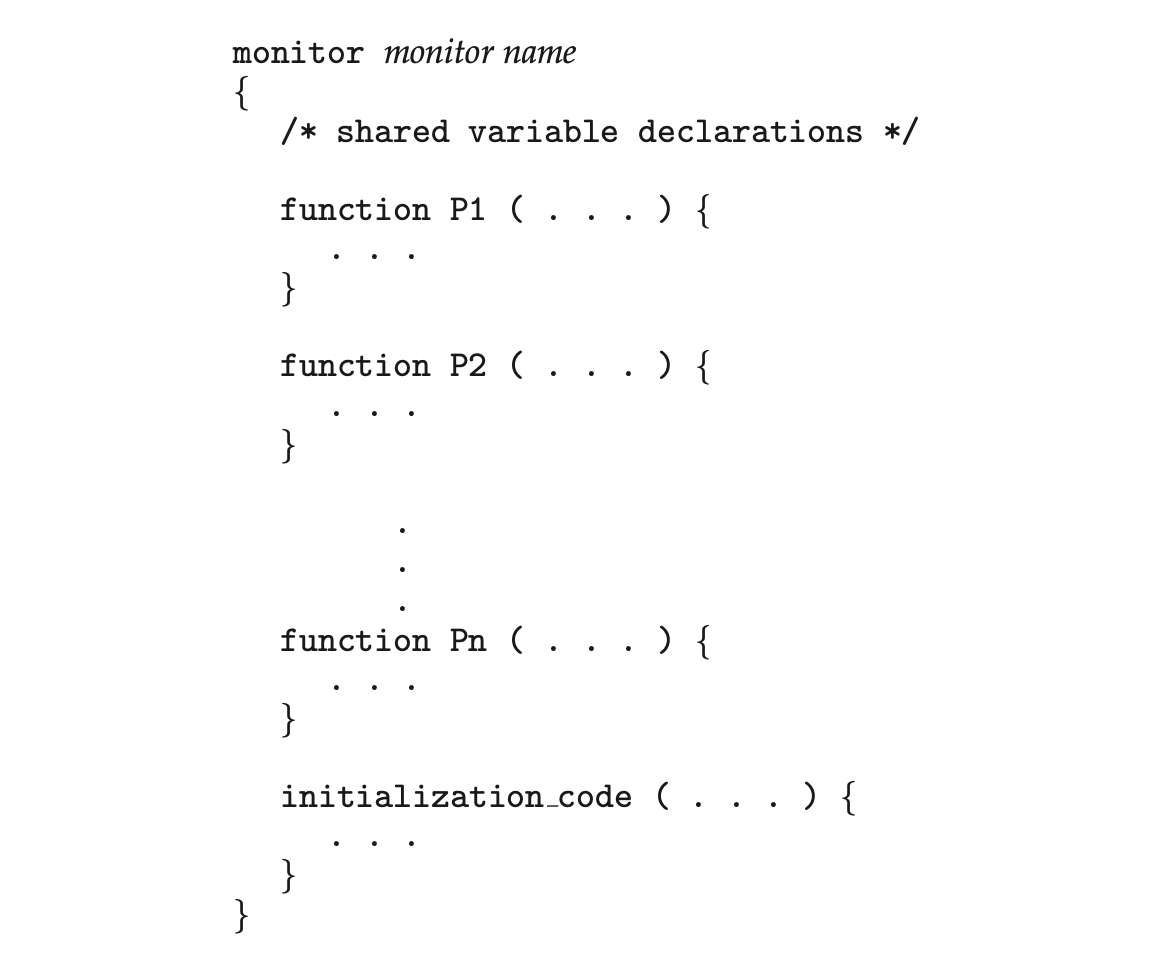
\includegraphics[width=\textwidth]{Pictures/monitorPseudocode.png}
	\caption{Struttura di un monitor in pseudocodice.}
\end{figure}
Le variabili dichiarate in un monitor formano lo \textbf{stato} del monitor e le funzioni definite nel monitor possono accedere solamente alle variabili dello stato, oltre che a quelle dichiarate localmente alla funzione ovviamente. Il monitor garantisce inoltre che un solo processo alla volta possa essere attivo all'interno del monitor (mutua esclusione).
Il monitor è provvisto di un ulteriore meccanismo di sincronizzazione dato dal costrutto \emph{condition}. Le uniche operazioni che possono essere invocate su una variabile condition sono \emph{wait()} e \emph{signal()}, le quali si comportano in maniera simile alle operazioni \emph{P()} e \emph{V()} dei semafori. Tuttavia \emph{wait()} blocca \textbf{sempre} il processo che la chiama e \emph{signal()} svaglia esattamente un solo processo, se non c'è nessun processo in attesa non succede nulla. Nel caso di \emph{signal} ci sono due comportamenti possibili:
\begin{itemize}
	\item \textbf{Signal and wait}. Il processo che ha chiamato signal attende e l'esecuzione passa al processo che si è sbloccato.
	\item \textbf{Signal and continue}. Il processo che ha chiamato signal continua la sua esecuzione ed esce dal monitor (in questo caso signal deve essere l'ultima istruzione della procedura).
\end{itemize}

Per concludere la trattazione sui monitor bisogna evidenziare come, sebbene essi siano più semplici da utilizzare per il programmatore, pochi linguaggi li implementano e per funzionare necessitino di memoria condivisa.

\section{Classi syncronized in Java}
Java come linguaggio ad alto livello fornisce un suo meccanismo per la sincronizzazione dei processi ovvero la keyword \emph{\textbf{syncronized}}.
Un metodo \emph{syncronized} è un metodo che può essere eseguito da una sola thread alla volta. Ciò viene realizzato mantendendo un singolo lock (detto monitor, ma da non confondere con i monitor trattati in precedenza) per oggetto. Se il metodo \emph{syncronized} è statico allora il lock viene messo sulla classe.
E' possibile inoltre definire una sezione critica su qualsiasi blocco utilizzando sempre la keyword \emph{syncronized}.
Sono disponibili inoltre altri metodi di sincronizzazione disponibili nella classe Object e quindi ereditati da tutti gli oggetti, ovvero \emph{\textbf{wait()}, \textbf{notify()}, \textbf{notifyAll()}}.

\chapter{Scheduling CPU}
Si intende per scheduling l'assegnazione di attivit\`a nel tempo: l'utilizzo della multiprogrammazione impone l'esistenza di una strategia per regolamentare l'ammissione dei processi
nel sistema e l'ammissione dei processi all'esecuzione. 
\section{Tipi di scheduling}
Gli scheduler si dividono in a lungo termine (job scheduler) che seleziona quali processi devono essere portati dalla memoria alla ready queue e gli scheduler a breve termine (CPU 
scheduler) che seleziona quale processo deve essere eseguito dalla CPU.
\subsection{Caratteristiche degli scheduler}
Lo scheduler a breve termine \`e invocato spesso e pertanto deve essere veloce, mentre lo scheduler a lungo termine \`e invocato pi\`u raramente e pu\`o essere pi\`u lento in quanto
controlla il grado di multiprogrammazione e il mix di processi. Il secondo pu\`o essere I/O bound con molto I/O e molti brevi burst di CPU o CPU-bound, con molti calcoli e pochi lunghi
burst di CPU. In sistemi con risorse limitate lo scheduler pu\`o essere assente. 
\subsection{Scheduling a medio termine}
I sistemi operativi con memoria virtuale prevedono un livello intermedio di scheduling per la momentanea rimozione forzata (swapping) di un processo dalla CPU per ridurre il grado di 
multiprogrammazione.
\section{Scheduling della CPU}
Il CPU scheduler \`e un modulo del sistema operativo che seleziona un processo tra quelli in memoria pronti per l'esecuzione e gli alloca la CPU e data la frequenza di invocazione \`e
una parte critica del sistema operativo in quanto necessita algoritmi di scheduling.
\subsection{Dispatcher}
Il dispatcher \`e un modulo del sistema operativo che passa il controllo della CPU al processo scelto dallo scheduler: fa lo switch del contesto, il passaggio alla modalit\`a user e 
il salto alla opportuna locazione nel programma per farlo ripartire. Nasce una latenza di dispatch, il tempo necessario al dispatcher per fermare un processo e farne ripartire un altro.
Deve pertanto essere la pi\`u bassa possibile. 
\subsection{Modello astratto del sistema}
Nel sistema si trova un alternanza di burst (sequenza) di CPU e I/O. Nel modello a cicli di burst CPU-I/O l'esecuzione di un processo  consiste dell'alternanza ciclica di un burst di CPU
e di uno di I/O. I CPU burst sono distribuiti esponenzialmente con molti burst brevi o pochi lunghi. 
\subsection{Prelazione (preemption)}
Si intende per prelazione il rilascio forzato della CPU. Quando non \`e presente il processo che detiene la CPU non la rilascia fino al termine del burst, mentre quando \`e presente 
pu\`o essere forzato a rilasciarla prima del termine. 
\subsection{Metriche di scheduling}
Per misurare la qualit\`a dello scheduling si considerano:
\begin{itemize}
	\item Utilizzo della CPU, con l'obiettivo di tenerla pi\`u occupata possibile.
	\item Throughput, il numero di processi completati per unit\`a di tempo.
	\item Tempo di attesa ($t_w$), la quantit\`a di tempo totale spesa da un processo nella coda di attesa influenzato dall'algoritmo di scheduling.
	\item Tempo di completamento (turnaround $t_t$), il tempo necessario ad eseguire un particolare processo dal momento della sottomissione al momento del completamento.
	\item Tempo di risposta ($t_r$), il tempo trascorso da quando una richiesta \`e stata sottoposta al sistema fino alla prima risposta del sistema spesso.
\end{itemize}
Per ottimizzare lo scheduling si deve pertanto massimizzare l'utilizzo della CPU e il throughput e minimizzare i tempi di turnaround, attesa e risposta.
\section{Algoritmi di scheduling}
\subsection{First-Come, First-Served (FCFS)}
La coda dei processi \`e una coda FIFO e il primo processo arrivato \`e il primo ad essere servito, ha un'implementazione semplice. Uno svantaggio ovvio \`e il cosiddetto effetto
convoglio: i processi brevi si accodano a processi lunghi preesistenti e sorgono problemi in contesti interattivi. 
\subsection{Shortest-Job-First (SJF)}
Associa ad ogni processo la lunghezza del prossimo burst di CPU e il processo con il burst pi\`u breve viene selezionato per l'esecuzione. Ne esistono due schemi uno non preemptive e uno
preemptive in cui se arriva un nuovo processo con un burst di CPU pi\`u breve del tempo che rimane da seguire al processo un esecuzione questo viene rimosso dalla CPU per fare spazio
a quello appena arrivato (algoritmo di shortest-remaining-time-first SRTF). SJF \`e ottimo in quanto permette il minimo tempo medio di attesa. 
\subsubsection{Calcolo del prossimo burst di CPU}
Di questo \`e possibile solo una stima utilizzando le lunghezze dei burst precedenti come proiezione di quelli futuri e utilizzando una media esponenziale: sia $t_n$ la lunghezza reale
dell'n-esimo burst, $\tau_{n+1}$ il valore stimato per il prossimo burst e $\alpha$ un coefficiente tale che $0<\alpha<1$, allora: 
$$\tau_{n+1} = \alpha\cdot t_n + (1-\alpha)\cdot \tau_n$$
Se $\alpha = 0$ la storia recente non viene utilizzata e se $\alpha = 1$ conta solo l'ultimo burst reale. Si nota come ogni termine successivo pesa meno del predecessore.
\subsection{Scheduling a priorit\`a}
In questo algoritmo viene associata una priorit\`a a ogni processo e la CPU viene allocata al processo con priorit\`a pi\`u alta. Pu\`o essere preemptive o non-preemptive. Si noti
come SJF \`e uno scheduing a priorit\`a data da $\frac{1}{\text{lunghezza del burst successivo}}$. Il comando \emph{nice} in Linux modifica la priorit\`a. Le politiche di assegnamento
della priorit\`a possono essere interne al sistema operativo (limiti di tempo, requisiti di memoria, numero di file aperti) o esterne (importanza del processo, motivi economici o 
politici). Pu\`o nascere il problema di starvation in quanto processi a bassa priorit\`a possono non essere mai eseguiti, risolti con un aumento della priorit\`a con il passare del
tempo. 
\subsection{Higher response ratio next (HRRN)}
\`E un algoritmo a priorit\`a non-preentive: la priorit\`a $$R=\frac{t_{attesa} + t_{burst}}{t_{burst}} = 1 + \frac{t_{attesa}}{t_{burst}}$$ \`e maggiore per valori di $R$ pi\`u alti e
dipende anche dal tempo di attesa e pertanto va ricalcolata al termine di un processo se nel frattempo ne sono arrivati altri o alt ermine di un processo. Supera il favoritismo di SJF
verso i job corti favorendo i processi che completano in poco tempo o quelli che hanno atteso molto. 
\subsection{Round robin (RR)}
Questo algoritmo basa lo scheduling su time-out: a ogni processo viene assegnato un quanto del processo di CPU tra i $10$ e i $100$ millisecondi e al termine del quanto il processo \`e
prelazionato e messo nella ready queue, una coda circolare. Se ci sono $n$ processi nella coda e il quanto \`e $q$ ogni processo ottiene $\frac{1}{n}$ del tempo di CPU in blocchi di 
$q$ unit\`a di tempo alla volta e nessun processo attende pi\`u di $(n-1)1$ unit\`a di tempo. \`E di semplice implementazione (FCFS con prelazione) il quanto va scelto con cura: 
se troppo grande diventa equivalente a FCFS, se troppo piccolo nasce troppo overhead per il context switch, un valore ragionevole \`e uno tale che l'$80\%$ dei burst siano minori di $q$.
Il tempo di turnaround \`e maggiore o uguale di SJF e quello di risposta minore o uguale di SJF. 
\subsection{Code multilivello}
\`E una classe di algoritmi in cui la ready queue \`e partizionata in pi\`u code e ogni coda ha il suo algoritmo di scheduling. Si rende necessario anche uno scheduling tra code, che
pu\`o essere a priorit\`a fissa con la possibilit\`a di starvation per le code a priorit\`a bassa o basato su time slice in cui ogni coda ottiene un quanto di tempo di CPU che pu\`o 
usare per schedulare i suoi processi. 
\subsection{Code multilivello con feedback}
Sono code multilivello in cui un processo pu\`o spostarsi da una coda all'altra a seconda delle sue caratteristiche (usato anche per implementare l'aging). Lo scheduler ha come parametri
il numero delle code, gli algoritmi per ogni coda, criteri per la promozione o degradazione di un processo e i criteri per definire la coda di ingresso di un processo. 
\subsection{Scheduling fair share}
Si noti come le politiche precedenti di scheduling sono orientate al processo ma non alle applicazioni (che possono essere composte da pi\`u processi). Fair share tenta di fornire
equit\`a alle applicazioni le vengono suddivise tra gruppi di processi (le applicazioni). 
\subsection{Valutazione degli algoritmi}
\subsubsection{Modello deterministico (analitico)}
Questa valutazione \`e basata sull'algoritmo e su un preciso carico di lavoro, definisce le prestazioni di ogni algoritmo per tale carico specifico. Vengono utilizzate per illustrare 
gli algoritmi e richiedono conoscenze troppo specifiche sulla natura dei processi. 
\subsubsection{Modello a reti di code}
Non esiste un preciso gruppo di processi per utilizzare il modello deterministico ma \`e possibile determinare le distribuzioni di CPU e I/O burst. Il sistema di calcolo \`e descritto 
come una rete di server ognuno con la propria coda e si usano formule matematiche che indicano la probabilit\`a che si verifichi un determinato CPU burst e la distribuzione dei 
tempi di arrivo nel sistema dei processi da cui \`e possibile ricavare utilizzo, throughput medio, tempi di attesa e altri parametri. 
\subsubsection{Simulazione}
Si programma un modello del sistema utilizzando dati statistici o reali (precisa ma costosa).
\subsubsection{Implementazione}
\`E l'unico modo sicuro per valutare un algoritmo di scheduling: lo si codifica, inserisce nel sistema operativo e si vede come funziona. 

\chapter{Sincronizzazione tra processi}
Il modello astratto della sincronizzazione tra processi \`e quello del produttore-consumatore: il primo produce un messaggio e il secondo lo consuma in esecuzione concorrente. Essendo il
buffer limitato ci sono dei vincoli: non si pu\`o aggiungere in buffer pieni e non si pu\`o consumare da buffer vuoti.
\subsection{Buffer: modello software}
In software il buffer \`e circolare di $N$ posizioni, con $in$ che indica la prima posizione libera e $out$ la prima posizione occupata. Il buffer \`e vuoto quando $in=out$ e pieno 
quando $out = (in + 1) \% n$. Per semplicit\`a si utilizza una variabile counter per indicare il numero di elementi nel buffer. Il produttore svolger\`a la sua operazione incrementando
il counter se e solo se il counter \`e minore di $N$ e il consumatore lo decrementa solo se \`e maggiore di $0$. Essendo le operazioni di incremento e decremento non atomiche (sono pi\`u
istruzioni assembly) non \`e noto l'ordine di interleaving tra i processi e possono nascere delle inconsistenze in quanto produttore e consumatore possono modificare \emph{counter}
contemporaneamente. Si rende necessario proteggere l'accesso alla sezione critica. 
\subsection{Sezione critica}
Si intende per sezione critica una porzione di codice in cui si accede ad una risorsa condivisa. La soluzione al suo problema deve rispettare:
\begin{itemize}
	\item Mutua esclusione: unicamente un processo alla volta pu\`o accedere alla sezione critica.
	\item Progresso: solo i processi che stanno per entrare nella sezione critica possono decidere chi entra e la decisione non pu\`o essere rimandata all'infinito.
	\item Attesa limitata: deve esistere un massimo numero di volte per cui un processo pu\`o aspettare di seguito.
\end{itemize}
Un generico processo che accede ad una risorsa condivisa ha una struttura che contiene un'operazione ripetuta contenente prima delle operazioni sulla sezione critica le regole di 
ingresso alla sezione critica, le operazioni su di essa, una sezione di uscita dalla stessa e successivamente le operazioni sulla sezione non critica.
\subsubsection{Soluzione}
Assumendo una sincronizzazione in ambiente globale con condivisione di celle di memoria, le soluzioni software riguardano aggiunta di codice alle applicazioni senza nessun supporto 
hardware o del sistema operativo, mentre le soluzioni hardware riguardano codice alle applicazioni con supporto hardware. 
\section{Soluzioni software}
\lstinputlisting[caption={PROCESS i}, language={C}]{Algoritmi/IPC-algoritmo1.c}
Questo algoritmo richiede stretta alternanza tra i processi: possono entrare nella zona critica unicamente alternativamente. Inoltre non rispetta il criterio del progresso in quanto
non esiste alcuna nozione di stato.
\subsection{Algoritmo 2}
\lstinputlisting[caption={PROCESS i}, language={C}]{Algoritmi/IPC-algoritmo2.c}
Risolve il problema dell'algoritmo 1 ma l'esecuzione in sequenza dell'istruzione \emph{flag[] = true} da parte dei due processi porta a deadlock. Invertendo le istruzioni della sezione
di entrata si viola la mutua esclusione in quanto entrambi i processi possono trovarsi nella sezione critica se eseguono in sequenza il \emph{while} prima di impostare la \emph{flag} a
\emph{true}
\subsection{Algoritmo 3}
\lstinputlisting[caption={PROCESS i}, language={C}]{Algoritmi/IPC-algoritmo3.c}
\`E la soluzione corretta in quanto entra il primo processo che esegue \emph{turn = j} oppure \emph{turn = i}
\subsubsection{Dimostrazione}
\paragraph{Mutua esclusione}
$P_i$ entra nella sezione critica se e solo se $flag[j] = false$ o $turn = i$. Se $P_i$ e $P_j$ sono entrambi nella sezione critica allora $flag[i]=flag[j]=true$, ma $P_i$ e $P_j$ non
possono aver superato entrambi il \emph{while} perch\`e $turn$ vale $i$ oppure $j$, pertanto solo uno dei due $P$ \`e entrato. 
\paragraph{Progresso e attesa limitata}
Se $P_j$ non \`e pronto per entrare nella sezione critica allora $flag[j]=false$ e $P_i$ pu\`o entrare. Se $P_j$ ha impostato $flag[j]=true$ e si trova nel \emph{while} allora $turn = i$
oppure $turn = j$. Se $turn = i$ $P_i$ entra nella sezione critica, se $turn = j$ vi entra $P_j$. In ogni caso quando $P_j$ esce dalla sezione critica imposta $flag[j]=false$ e 
quindi $P_i$ pu\`o entrare nella sezione critica e $P_i$ entra nella sezione critica al massimo dopo un'entrata di $P_j$. 
\subsection{Algoritmo del fornaio}
Risolve il problema con $N$ processi: ogni processo sceglie un numero (\emph{choosing[i] = l}), il numero pi\`u basso viene servito per primo e per situazioni di numero identico si
usa un confronto a due livelli (\emph{numero, i}). L'algoritmo \`e corretto. 
\lstinputlisting[caption={PROCESS i}, language={C}]{Algoritmi/IPC-algoritmo-fornaio.c}
\section{Soluzioni hardware}
Un modo hardware per risolvere il problema della sezione critica \`e di disabilitare gli interrupt mentre una variabile condivisa viene modificata. Da questo nasce un problema in quanto
se il test per l'accesso \`e lungo gli interrupt devono essere disabilitati per troppo tempo. Un'alternativa \`e che l'operazione per l'accesso alla risorsa deve occupare un unico ciclo
di istruzione non interrompibile, con istruzioni atomiche di \emph{Test-and-set} e \emph{swap}
\subsection{Test and Set}
\lstinputlisting[caption={Test and Set}, language={C}]{Algoritmi/Test_and_set.c}
Il valore di ritorno \`e il valore di \emph{var} a cui viene assegnato \emph{true}. Si passa a questa funzione un lock che permette il controllo della sezione critica a un processo alla 
volta in quanto passa solo il primo processo che arriva e trova \emph{lock = false}. Quando il processo termina le operazioni sulla sezione critica pone \emph{lock = false}.
\subsection{Swap}
\lstinputlisting[caption={Swap}, language={C}]{Algoritmi/Swap.c}
Lo \emph{swap} viene utilizzato sul \emph{lock} e una variabile locale, che permette l'accesso solo quando quella locale diventa \emph{false} in modo da eliminare la competizione sul
\emph{lock}. Si noti come \emph{TestAndSet} e \emph{Swap} non rispettano attesa limitata in quanto manca l'equivalente della variabile \emph{turn} e sono pertanto necessarie variabili
addizionali.
\subsection{Test and Set con attesa limitata}
\lstinputlisting[caption={PROCESS i}, language={C}]{Algoritmi/TestSetLimitata.c}
\subsection{Conclusioni}
I vantaggi delle soluzioni hardware sono la scalabilit\`a in quanto indipendenti dal numero di processi coinvolti e il fatto che l'estensione a $N$ sezioni critiche \`e immediato. 
Offrono per\`o maggiore complessit\`a al programmatore rispetto alle soluzioni software e serve busy waiting con spreco di CPU.
\section{Semafori}
Si nota come le soluzioni precedenti non sono banali da aggiungere a programmi e sono basate su busy waiting. I semafori offrono una soluzione generica che funziona sempre. Si intende
per semaforo una variabile intera $S$ a cui si accede attraverso due primitive atomiche: 
\begin{itemize}
	\item Signal: \emph{V(s)} che incrementa il valore di $S$ di $1$. 
	\item Wait: \emph{P(s)} che tenta di decrementare il valore di $S$ di $1$, se \`e $0$ non si pu\`o ed \`e necessario attendere.
\end{itemize}
Esistono i semafori in versione binaria (con $S$ $0$ o $1$) o generica (con $S$ a valori interi maggiori o uguali di $0$).
\subsection{Semafori binari} 
Si noti come i semafori binari abbiano lo stesso potere espressivo di quelli a valori interi.
\lstinputlisting[caption={Implementazione concettuale}, language={C}]{Algoritmi/SemBinCon.c}
\subsubsection{Con busy waiting}
\begin{multicols}{2}
	\lstinputlisting[caption={Semaforo binario}, language={C}]{Algoritmi/SemBinWBW-P.c}
	\columnbreak
	\lstinputlisting[caption={Semaforo binario}, language={C}]{Algoritmi/SemBinWBW-V.c}
\end{multicols}
\subsection{Semafori interi}
Il problema dei semafori interi \`e garantirne l'atomicit\`a. 
\lstinputlisting[caption={Implementazione concettuale}, language={C}]{Algoritmi/SemIntCon.c}
\subsubsection{Con busy waiting}
Sia \emph{bool mutex} un semaforo binario inizializzato a \emph{TRUE} e \emph{bool delay} un semaforo binario inizializzato a \emph{FALSE}. Sia in \emph{P} che in \emph{V} l'operazione
\emph{P(mutex)} protegge $S$ da un'altra modifica. In \emph{V} \emph{V(delay)} permette la liberazione di un processo in attesa. In \emph{P} se qualcuno occupa il semaforo si attende, 
altrimenti lo si passa. 
\begin{multicols}{2}
	\lstinputlisting[caption={Semaforo intero}, language={C}]{Algoritmi/SemIntWBW-P.c}
	\columnbreak
	\lstinputlisting[caption={Semaforo intero}, language={C}]{Algoritmi/SemIntWBW-V.c}
\end{multicols}
\subsubsection{Senza busy waiting}
Nei semafori interi senza busy waiting si necessita di \emph{bool mutex}, un semaforo binario inizializzato a \emph{TRUE}. Inoltre il semaforo non \`e pi\`u un intero ma una 
\emph{struct} contenente un valore intero (con semantica analoga a quello con busy wating) e una lista contenente i PCB (process control block). Inoltre l'operazione di \emph{sleep()}
mette il processo nello stato di waiting mentre \emph{wakeup} lo mette nello stato ready. Si noti come si deve decidere l'ordine di \emph{wakeup} dei processi.
\lstinputlisting[caption={Semaforo intero}, language={C}]{Algoritmi/SemIntWoutBW.c}
\begin{multicols}{2}
	\lstinputlisting[caption={Semaforo intero}, language={C}]{Algoritmi/SemIntWoutBW-P.c}
	\columnbreak
	\lstinputlisting[caption={Semaforo intero}, language={C}]{Algoritmi/SemIntWoutBW-V.c}
\end{multicols}
In questo caso il busy waiting viene eliminato dalla entry section ma rimane nella \emph{P} e \emph{V} del mutex che essendo veloce porta a poco spreco di CPU. Un alternativa \`e 
disabilitare gli interrupt durante \emph{P} e \emph{V} in cui istruzioni di processi diversi non possono essere eseguite in modo alternato. 
\subsection{Implementazione}
Si noti come l'implementazione reale \`e diversa da quella concettuale: il valore di \emph{s} pu\`o diventare minore di zero per i semafori interi in quanto conta quanti processi ci 
sono in attesa. La lista dei PCB pu\`o essere FIFO (strong semaphore) garantendo cos\`i attesa limitata. Nella modalit\`a di implementazione con busy waiting (spinlock) la CPU controlla
attivamente il verificarsi della condizione di accesso alla sezione critica. \`E una soluzione scalabile e veloce, CPU-intensive e adatta per attese brevi, come l'accesso a memoria.
Nella modalit\`a senza busy waiting con sleep (mutex, semaforo) il processo viene messo inattesa che si verifichi la condizione di accesso alla sezione critica. \`E pi\`u lento e 
adatto per attese lunghe come l'I/O.
\subsection{Applicazioni}
Un semaforo binario con valore iniziale $1$ (mutex) viene utilizzato per la protezione di una sezione critica per $n$ processi. Un semaforo binario con valore iniziale $0$ viene 
utilizzato per la sincronizzazione del tipo di attesa di evento tra processi.
\subsubsection{Sezione critica}
Si dice mutex un semaforo binario di mutua esclusione. In questo caso $n$ processi condividono la variabile $s$.
\lstinputlisting[caption={Mutex}, language={C}]{Algoritmi/SemBinSezCrit.c}
\subsubsection{Semafori per attesa evento}
Si consideri il caso di due processi $P1$ e $P2$ che devono sincronizzarsi rispetto all'esecuzione di due operazioni $A$ e $B$ in modo che $P2$ possa eseguire $B$ solo dopo che $P1$
ha eseguito $A$. In questo caso si usa un semaforo binario $s$ inizializzato a $0$ tale che $P1$ svolga \emph{V(s)} dopo $A$ e $P2$ svolga $B$ dopo \emph{P(s)}.\\
Si consideri il caso di due processi $P1$ e $P2$ che devono sincronizzarsi rispetto all'esecuzione di un'operazione $A$ in maniera alternata. Vengono pertanto utilizzati due semafori 
$s1$ inizializzato a $1$ e $s2$ inizializzato a $0$ in modo che $P1$ svolga \emph{P(s1)} prima di $A$ e \emph{V(s2)} dopo, mentre $P2$ \emph{P(s2)} prima e \emph{V(s1)} dopo. 
\subsection{Limitazioni}
I semafori possono generare deadlock, in cui il processo viene bloccato in attesa di un evento che solo lui pu\`o generare o starvation, in cui avviene un'attesa indefinita all'interno
del semaforo. 
\section{Problemi classici dei semafori}
\subsection{Produttore consumatore}
Il problema del produttore consumatore consiste di due processi con accesso sullo stesso buffer di dimensione limitata. Il produttore scrive nel buffer  mentre il consumatore legge e
lo svuota. IL problema richiede tre semafori:
\begin{itemize}
	\item Mutex, un semaforo binario inizializzato a \emph{TRUE} che garantisce la mutua esclusione per il buffer.
	\item Empty, un semaforo intero inizializzato a $N$ che blocca $P$ se il buffer \`e pieno.
	\item Full, un semaforo intero inizializzato a $0$ che blocca $C$ se il buffer \`e vuoto.
\end{itemize}
\newpage
\begin{multicols}{2}
	\lstinputlisting[caption={Produttore}, language={C}]{Algoritmi/Produttore.c}
	\columnbreak
	\lstinputlisting[caption={Consumatore}, language={C}]{Algoritmi/Consumatore.c}
\end{multicols}
\subsection{Dining philosophers}
Si considerino $N$ filosofi che passano la vita mangiando e pensando. Si trova $1$ tavola con $N$ bacchette e una ciotola di riso. Se un filosofo pensa non interagisce con gli altri.
Se un filosofo ha fame prende $2$ bacchette e inizia a mangiare. Il filosofo pu\`o prendere solo le bacchette che sono alla sua destra e alla sua sinistra e pu\`o prenderne solo una 
alla volta. Se non ci sono due bacchette libere non pu\`o mangiare. Quando un filosofo termina di mangiare rilascia le bacchette.
\subsubsection{Prima soluzione}
\begin{multicols}{2}
	\paragraph{Dati condivisi}
	\begin{itemize}
		\item Ci sono $n$ semafori $s[N]$ inizializzati a $1$.
		\item $P(s[j])$ vuol dire che si cerca di prendere la bacchetta $j$;
		\item $V(s[j])$ rilascia la bacchetta $j$>
	\end{itemize}
	\paragraph{La soluzione \`e incompleta} C'\`e un possibile deadlock se tutti i filosofi tentano di prendere la bacchetta alla loro destra (sinistra) contemporaneamente. 
	\columnbreak
	\lstinputlisting[caption={Dining philosopher}, language={C}]{Algoritmi/Philosopher1.c}
\end{multicols}
\paragraph{Deadlock}
Questa soluzione presenta un problema in quanto nasce un deadlock nel caso in cui ogni filosofo prende la bacchetta di destra e si trovano tutti ad aspettare che si liberi quella di 
sinistra che nessuno pu\`o rilasciare. 
\paragraph{Possibili soluzioni parziali}
\begin{itemize}
	\item Si permette solo a quattro filosofi di mangiare contemporaneamente.
	\item Soluzione asimmetrica in cui i filosofi in posizione pari prendono la bacchetta sinistra seguita dalla destra mentre i filosofi in posizione dispari fanno il contrario.
	\item I filosofi si passano un token.
	\item Si permette ai filosofi di prendere la bacchetta solo se sono entrambe disponibili.
\end{itemize}
\subsubsection{Soluzione corretta}
In questa soluzione ogni filosofo si pu\`o trovare in tre stati: pensante (\emph{THINKING}), affamato (\emph{HUNGRY}) e  mangiante (\emph{EATING}). Le variabili condivise sono un 
semaforo mutex inizializzato a $1$ $N$ semafori $f[N] = 0$ e lo stato di ogni filosofo $stato[N]$. 
\begin{multicols}{2}
	\lstinputlisting[caption={Dining philosopher}, language={C}]{Algoritmi/Philosopher2.c}
	\lstinputlisting[caption={Test}, language={C}]{Algoritmi/Philosopher2-test.c}
	\columnbreak	
	\lstinputlisting[caption={Drop fork}, language={C}]{Algoritmi/Philosopher2-dropfork.c}
	\lstinputlisting[caption={Take fork}, language={C}]{Algoritmi/Philosopher2-takefork.c}
\end{multicols}
\subsection{Sleepy barber}
Un negozio ha una sala d'attesa con $N$ sedie ed una stanza con la sedia del barbiere. In assenza di clienti il barbiere si addormenta. Quando entra un cliente se le sedie sono 
occupate il cliente se ne va, se il barbiere \`e occupato si siede e se \`e addormentato lo sveglia. 
\subsubsection{Soluzione}
\paragraph{Dati condivisi}
\begin{itemize}
	\item Semaforo intero customer inizializzato a zero che sveglia il barbiere.
	\item Semaforo binario barbers inizializzato a zero che rappresenta lo stato del barbiere.
	\item Semaforo binario mutex inizializzato a $1$ che protegge la sezione critica.
	\item \emph{int waiting = 0} che conta i clienti in attesa.
\end{itemize}
\begin{multicols}{2}
	\lstinputlisting[caption={Barber}, language={C}]{Algoritmi/Barber.c}
	\columnbreak
	\lstinputlisting[caption={Consumer}, language={C}]{Algoritmi/Customer.c}
\end{multicols}
\subsection{Limitazioni dei semafori}
L'utilizzo dei semafori presenta delle difficolt\`a in quanto risulta difficile scrivere programmi e la correttezza delle soluzioni \`e difficilmente dimostrabile. In alternativa 
vengono pertanto utilizzati specifici costrutti forniti da linguaggi di programmazione ad alto livello come monitor, classi synchronized in Java e CCR (conditional critical region) e 
altri. 
\section{Monitor}
Sono costrutti per la condivisione sicura ed efficiente di dati da processi. Sono simili al concetto di classe.
\lstinputlisting[caption={Monitor}, language={C}]{Algoritmi/Monitor.c}
Le variabili del monitor sono visibili solo all'interno del monitor stesso e le procedure del monitor accedono solo alle variabili definite nel monitor. Un solo processo alla volta 
risulta attivo in un monitor in modo che il programmatore non debba codificare esplicitamente la mutua esclusione. 
\subsection{Operazioni del monitor}
Per permettere ad un processo di attendere all'interno del monitor si rendono necessari opportune sincronizzazioni: le variabili condition dichiarate all'interno del monitor e 
accessibili solo tramite due primitive analoghe a quelle dei semafori: \emph{wait()} come \emph{P()} e \emph{signal()} come \emph{V()}. Il processo che invoca \emph{x.wait()} \`e 
bloccato fino all'invocazione della corrispondente \emph{x.signal()} da parte di un altro. 
\subsubsection{Wait}
La \emph{wait} blocca sempre il processo che la chiama e si deve pertanto prestare attenzione alla logica che regola tale chiamata. 
\subsubsection{Signal}
La \emph{signal} sveglia esattamente un processo e se ne trovano pi\`u in attesa lo scheduler decide quale processo pu\`o entrare. Se nessun processo si trova in attesa non c'\`e nessun
effetto. Successivamente a questa operazione il processo che la invoca si pu\`o bloccare passando l'esecuzione al processo sbloccato o esce dal monito, caso in cui signal deve essere
l'ultima istruzione di una procedura. 
\subsubsection{Buffer produttore consumatore}
\begin{multicols}{2}
	\lstinputlisting[caption={Produttore}, language={C}]{Algoritmi/MonitorProduttore.c}
	\columnbreak
	\lstinputlisting[caption={Consumatore}, language={C}]{Algoritmi/MonitorConsumatore.c}
\end{multicols}
\lstinputlisting[caption={Monitor per buffer}, language={C}]{Algoritmi/MonitorProducerConsumer.c}
\subsubsection{Semaforo binario nel monitor}
\lstinputlisting[caption={Semaforo binario nel monitor}, language={C}]{Algoritmi/MonitorSemBin.c}
\subsection{Limitazioni}
Pur essendo meno proni ad errori rispetto ai semafori i monitor sono forniti da pochi linguaggi e richiedono sempre presenza di memoria condivisa. 
\section{Sincronizzazione in Java}
La sezione critica viene indicata dalla keyword synchronized e i metodi synchronized possono essere eseguiti da un solo thread alla volta e vengono realizzati mantenendo un singolo lock
detto monitor per oggetto. I metodi static synchronized presentano un solo lock per classe, mentre per i blocchi synchronized \`e possibile mettere un lock su qualsiasi oggetto per 
definire una sezione critica. Altri metodi di sincronizzazione sono \emph{wait()} \emph{notify()} e \emph{notifyAll()}, che vengono ereditati da tutti gli oggetti. 
\subsection{Buffer produttore consumatore}
\begin{multicols}{2}
	\lstinputlisting[caption={Bounded buffer}, language={Java}]{Algoritmi/BoundedBuffer.java}
	\columnbreak
	\lstinputlisting[caption={Deposit}, language={Java}]{Algoritmi/Deposit.java}
	\lstinputlisting[caption={Remove}, language={Java}]{Algoritmi/Remove.java}
\end{multicols}
\section{Conclusioni}
IL problema della soluzione critica \`e un'astrazione della concorrenza tra processi. Esistono soluzioni con diversi compromessi tra complessit\`a e difficolt\`a di utilizzo. Si 
deve prestare attenzione alla gestione del blocco critico di un insieme di processi (deadlock) dipendente dalla sequenza temporale degli accessi.
\section{Problema degli scrittori e dei lettori}
C'\`e un area di dati condivisa ed esistono dei lettori che possono solo leggere i dati e scrittori che possono solo scriverli. Pi\`u lettori possono leggere il file contemporaneamente, 
solo uno scrittore alla volta pu\`o scrivere nel file, se uno scrittore sta scrivendo nel file nessun lettore pu\`o leggerlo, gli scrittori non possono leggere e i lettori non possono
essere anche scrittori. 
\lstinputlisting[caption={Scrittore}, language={C}]{Algoritmi/Scrittore.c}
\lstinputlisting[caption={Lettore}, language={C}]{Algoritmi/Lettore.c}

\chapter{Deadlock}
In una sequenza di utilizzo dei processi che utilizzano risorse si trovano tre fasi:
\begin{itemize}
	\item Richiesta: se non pu\`o essere immediatamente soddisfatta il processo deve attendere.
	\item Utilizzo.
	\item Rilascio.
\end{itemize}
Un insieme di processi si definisce in deadlock quando ogni processo \`e in attesa di un evento che pu\`o essere causato solo da un processo dello stesso insieme. Un deadlock si pu\`o 
risolvere attraverso preemption e rollback, con pericolo di starvation. 
\subsection{Condizioni necessarie}
Affinch\`e si verifichi un deadlock devono essere vere contemporaneamente:
\begin{itemize}
	\item Mutua esclusione: almeno una risorsa deve essere non condivisibile.
	\item Hold and Wait: deve esistere un processo che detiene una risorsa e che attende di acquisirne un'altra detenuta da un altro. 
	\item No preemption: le risorse non possono essere rilasciate se non volontariamente dal processo che le usa.
	\item Attesa circolare: deve esistere un insieme di processi che attendono ciclicamente il liberarsi di una risorsa. 
\end{itemize}
\section{Modello astratto: resource allocation graph (RAG)}
Sia un RAG un grafo $G(V, E)$ tale che i nodi $V$ rappresentati attraverso cerchi sono i processi mentre i nodi rappresentati come rettangoli sono le risorse. Nei rettangoli si trovano
tanti cerchi quante sono le istanze della corrispondente risorsa. Gli archi $E$ da processi a risorse indicano un processo che richiede una risorsa, mentre da risorse a processi 
indicano che il processo detiene la risorsa. Se il RAG non contiene cicli non ci sono deadlock, mentre se ne contiene se si ha una sola istanza per risorsa allora si ha deadlock, 
mentre se ci sono pi\`u istanze dipende dallo schema di allocazione. 
\section{Gestione dei deadlock}
\subsection{Prevenzione statica}
Nella prevenzione statica si tenta di evitare che si possa verificare una delle quattro condizioni. 
\subsubsection{Mutua esclusione}
Si noti come la mutua esclusione \`e irrinunciabile per certi tipi di risorsa e pertanto non \`e risolvibile.
\subsubsection{Hold and Wait}
Una soluzione consiste nel fatto che un processo alloca all'inizio tutte le risorse che deve utilizzare o pu\`o ottenerne una solo se non ne ha altre. Con queste soluzioni si ottiene
un basso utilizzo delle risorse con possibilit\`a di starvation in caso di richiesta di molte risorse molto popolari. Si deve inoltre conoscere il numero di risorse richieste. 
\subsubsection{No preemption}
Una soluzione consiste nel fatto che un processo che richiede una risorsa non disponibile deve cedere tutte le altre risorse che detiene. In alternativa pu\`o cedere risorse che 
detiene su richiesta di un altro processo. Si noti come \`e fattibile solo per risorse il cui stato pu\`o essere ristabilito facilmente. 
\subsubsection{Attesa circolare}
Si assegna una prioriit\`a, un ordinamento globale ad ogni risorsa in modo che un processo pu\`o richiedere risorse solo in ordine crescente di priorit\`a, pertanto l'attesa circolare
diventa impossibile. La priorit\`a deve seguire il normale ordine di richiesta. 
\subsection{Prevenzione dinamica (avoidance)}
Questo metodo si basa sull'allocazione delle risorse e non viene mai utilizzata poich\`e richiede una conoscenza troppo approfondita delle richieste di risorse. Si noti come le 
tecniche di prevenzione statica possono portare a un basso utilizzo delle risorse perch\`e mettono vincoli sul modo in cui i processi possono accedere alle risorse. L'obiettivo \`e la
prevenzione in base alla richieste: un analisi dinamica del grafo delle risorse per evitare situazioni cicliche. Richiede come requisito la conoscenza del caso peggiore: il massimo 
numero di istanze di una risorsa richieste per processo. 
\subsubsection{Stato Safe}
Lo stato di assegnazione delle risorse viene calcolato come il numero di istanze disponibili e allocate e le richieste massime dei processi. Il sistema si trova in uno stato sicuro
se esiste una sequenza safe ovvero se usando le risorse disponibili pu\`o allocare risorse ad ogni processo in qualche ordine in modo che ciascuno di essi possa terminare la sua
esecuzione. 
\subsubsection{Sequenza Safe}
Una sequenza di processi $(P_1, \dots, P_N)$ \`e safe se per ogni $P_i$ le risorse che $P_i$ pu\`o richiedere possono essere esaudite usando le risorse disponibili e quelle detenute da
$P_j$, $j < i$, ovvero attendendo che $P_j$ termini. Se non esiste tale sequenza si trova in uno stato unsafe. Si noti come non tutti gli stati unsafe sono deadlock, ma da stato 
unsafe si pu\`o arrivare ad un deadlock. 
\subsubsection{Metodo della prevenzione dinamica}
Si usano algoritmi che lasciano il sistema sempre in uno stato safe. All'inizio il sistema \`e in uno stato safe. Ogni volta che $P$ richiede $R$, $R$ viene assegnata a $P$ se e solo
se si rimane in uno stato safe. L'utilizzo delle risorse sar\`a sempre minore rispetto al caso in cui non si usano tecniche di prevenzione dinamica. 
\subsubsection{Algoritmo con RAG}
Questo algoritmo funziona solo se c'\`e una sola istanza per risorsa. Il RAG viene esteso con archi di rivendicazione: $P_i\rightarrow R_j$ se $P_i$ pu\`o richiedere $R_j$ in futuro. 
Questi archi vengono indicati con una freccia tratteggiata. All'inizio ogni processo deve rendere noto quali risorse vorrebbe usare durante la sua esecuzione. Una richiesta viene 
soddisfatta se e solo se l'allocazione della risorsa non crea un ciclo nel RAG. Serve un algoritmo per la rilevazione dei calci di complessit\`a ($O(n^2)$, dove $n$ \`e il numero di 
processi)
\subsubsection{Algoritmo del banchiere}
Pure essendo meno efficiente dell'algoritmo con RAG funziona qualunque sia il numero di istanze. In questo algoritmo il banchiere non deve mai distribuire tutto il denaro che ha in cassa
in quanto altrimenti non potrebbe pi\`u soddisfare successivi clienti. Ogni processo dichiara la sua massima richiesta e ogni volta che un processo richiede una risorsa si determina se 
soddisfarla lascia uno stato safe. Tale algoritmo \`e costituito da un algoritmo di allocazione e uno di verifica dello stato. 
\lstinputlisting[caption={Strutture dati per $n$ processi e $m$ risorse}, language={C}]{Algoritmi/Banchierestrutture.c}
\paragraph{Algoritmo di allocazione}
\lstinputlisting[caption={Allocazione per $P_i$}, language={C}]{Algoritmi/BanchiereAllocazione.c}
\paragraph{Algoritmo di verifica dello stato}
\lstinputlisting[caption={Verifica dello stato}, language={C}]{Algoritmi/BanchiereVerifica.c}
Si noti come questo algoritmo abbia complessit\`a $O(m\cdot n^2)$.
\subsection{Rilevamento (detection) e ripristino (recovery)}
In questo metodo si permette che si verifichino deadlock e prevede metodi per riportare il sistema al funzionamento normale. Nasce in quanto prevenzione statica e dinamica sono 
conservativi e riducono eccessivamente l'utilizzo delle risorse. Ci sono due approcci alternativi: rilevamento del ripristino tramite il grafo di attesa calcolato attraverso il RAG
e l'algoritmo di rilevazione.
\subsubsection{Attraverso il RAG}
Funziona solo con una risorsa per tipo e consiste nell'analizzare periodicamente il RAG< verificare se esistono deadlock ed iniziare il ripristino. Non \`e necessaria una conoscenza
anticipata delle richieste e permette un loro utilizzo migliore ma presenta il costo del recovery. 
\subsubsection{Algoritmo di rilevamento}
L'algoritmo di rilevamento si basa sull'esplorazione di ogni possibile sequenza di allocazione per i processi che non hanno ancora terminato. Se la sequenza va a buon fine (\`e safe)
non avviene deadlock.
\lstinputlisting[caption={Strutture dati per $n$ processi e $m$ risorse}, language={C}]{Algoritmi/RilevamentoStrutture.c}
\lstinputlisting[caption={Algoritmo di rilevamento}, language={C}]{Algoritmi/RilevamentoAlgoritmo.c}
\subsubsection{Ripristino}
L'algoritmo di rilevamento pu\`o essere chiamato dopo ogni richiesta, ogni $N$ secondi o quando l'utilizzo della CPU scende sotto una soglia $T$ e pu\`o uccidere i processi coinvolti o 
fare prelazione delle risorse dai processi bloccati nel deadlock. 
\paragraph{Uccisione dei processi}
Questo approccio \`e costoso in quanto tutti i processi devono ripartire e perdono il lavoro svolto. Uccidere selettivamente fino alla scomparsa del deadlock \`e costoso in quanto
invoca l'algoritmo di rilevazione dopo ogni uccisione e si deve decidere accuratamente l'ordine. 
\paragraph{Prelazione delle risorse}
Il problema \`e che il processo che subisce la prelazione non pu\`o continuare normalmente e pertanto si deve fare rollback in uno stato safe da cui si riparte (eventualmente ripartendo
da zero). \`E possibile starvation se tolgo le risorse sempre agli stessi processo. Si deve pertanto considerare il numero di rollback nei fattori di costo. 
\subsection{Algoritmo dello struzzo}
In questo metodo non si fa nulla in quanto i deadlock sono rari e gestirli costa troppo. 
\section{Conclusioni}
Ognuno degli approcci ha vantaggi e svantaggi, nessuno superiore agli altri. Si pu\`o avere una soluzione combinata che partiziona le risorse in classi usando una strategia di 
ordinamento con l'algoritmo pi\`u appropriato per la classe.
\subsection{Partizionamento in classi}
\begin{enumerate}
	\item Risorse interne usate dal sistema.
	\item Memoria.
	\item Risorse di processo.
	\item Spazio di swap.
\end{enumerate}
\subsection{Algoritmi specifici}
\begin{enumerate}
	\item Prevenzione tramite ordinamento delle risorse.
	\item Prevenzione tramite prelazione: un job pu\`o essere swappato.
	\item Prevenzione dinamica: richiesta massima di risorse nota a priori.
	\item Prevenzione tramite preallocazione: richiesta massima nota a priori.
\end{enumerate}
\`E sempre possibile ignorare i deadlock in quanto sono eventi rari, la prevenzione \`e costosa come il recovery e gli algoritmi sono spesso sbagliati. 

\chapter{Gestione della memoria}
La condivisione della memoria da parte di pi\`u processi \`e essenziale per l'efficienza del sistema. Offre problematiche negli ambiti di allocazione della memoria ai singoli job, per
la protezione e condivisione dello spazio di indirizzamento e per la gestione della memoria virtuale (swap). Nei sistemi moderni la gestione della memoria \`e inseparabile dal concetto
di memoria virtuale. Ogni processo deve essere portato in memoria e trasformato in processo per essere eseguito. La CPU preleva le istruzioni da eseguire dalla memoria in base al
valore del program counter. L'istruzione viene codificata e pu\`o prevedere il prelievo di operandi dalla memoria. Al termine dell'istruzione il risultato pu\`o essere scritto in 
memoria. Quando il processo termina la sua memoria viene rilasciata. 
\section{Da programma a processo}
La trasformazione da programma a processo avviene attraverso varie fasi precedenti all'esecuzione: in ogni fase si ha una diversa semantica degli indirizzi (spazio logico e spazio
fisico). Gli indirizzi del programma sorgente sono simbolici e trasformati in indirizzi fisici attraverso il compilatore che associa agli indirizzi simbolici indirizzi rilocabili
e il linker o il loader associano agli indirizzi rilocabili indirizzi assoluti. Si noti come gli indirizzi hanno diverse rappresentazioni nelle varie fasi di costruzione di un programma.
Il collegamento tra indirizzi simbolici e fisici viene detto binding.
\subsection{Binding}
Il binding di dati e istruzioni a indirizzi di memoria pu\`o avvenire in tre momenti distinti:
\begin{enumerate}
	\item Tempo di compilazione: statico, se \`e noto a priori in quale parte della memoria risieder\`a il processo \`e possibile generare codice assoluto, ma se la locazione di 
		partenza cambia sar\`a necessario ricompilare.
	\item Tempo di caricamento: statico, si rende necessario generare codice rilocabile con indirizzi relativi all'inizio del programma. Se cambia indirizzo di riferimento si deve
		ricaricare. 
	\item Tempo di esecuzione: dinamico, il binding viene posticipato se il processo pu\`o essere spostato durante l'esecuzione in posizioni diverse della memoria. Viene richiesto 
		supporto hardware affinch\`e l'operazione possa essere fatta efficientemente. 
\end{enumerate}
\subsection{Collegamento}
Il collegamento pu\`o essere statico in cui tutti i riferimenti sono definiti prima dell'esecuzione e l'immagine del processo contiene una copia delle librerie usate o dinamico in cui il
link viene posticipato al tempo di esecuzione e il codice del programma non contiene il codice delle librerie ma solo un riferimento (stub) per poterle recuperare. 
\subsection{Caricamento}
Il caricamento pu\`o essere statico in cui tutto il codice viene caricato in memoria a tempo dell'esecuzione o dinamico in cui il caricamento dei moduli viene posticipato in 
corrispondenza del primo utilizzo (risulta utile per codice con molti casi speciali).
\subsection{Spazi di indirizzamento}
Lo spazio di indirizzamento logico \`e legato a uno spazio di indirizzamento fisico: l'indirizzo logico (o virtuale) \`e generato dalla CPU mentre quello fisico viene considerato dalla
memoria. Nel binding a compile o load-time l'indirizzo fisico e logico coincidono mentre in quello a run-time sono generalmente diversi. 
\subsubsection{Memory management unit (MMU)}
La memory management unit \`e un dispositivo hardware che mappa indirizzi virtuali in indirizzi fisici: il valore del registro di rilocazione \`e aggiunto ad ogni indirizzo generato
da un processo e inviato alla memoria. 
\subsection{Considerazioni}
In un sistema multiprogrammato non \`e possibile conoscere in anticipo dove un processo pu\`o essere posizionato in memoria e lo swap impedisce di poter utilizzare indirizzi rilocati
in modo statico. Pertanto non \`e possibile il binding a tempo di compilazione o di caricamento. Si deve far affidamento alla rilocazione dinamica usata per sistemi complessi come la
gestione della memoria nel sistema operativo o la rilocazione statica, possibile in sistemi progettati per applicazioni specifiche e con limitata gestione della memoria nel sistema
operativo. 
\section{Schemi di gestione della memoria}
I metodi principali di gestione della memoria sono:
\begin{itemize}
	\item Allocazione contigua.
	\item Paginazione.
	\item Segmentazione.
	\item Segmentazione doppia.
\end{itemize}
Si noti come tutti prevedono che il programma sia interamente caricato in memoria, mentre soluzioni realistiche usano memoria virtuale. 
\subsection{Allocazione contigua}
Nell'allocazione contigua i processi sono allocati in memoria in posizioni contigue all'interno di una partizione. Le partizioni possono essere fisse o variabili. La memoria \`e un 
insieme di partizioni di dimensioni predefinite e diverse. Nascono problematiche per l'assegnazione di memoria ai job e per il supporto della rilocazione dinamica. L'assegnazione della
memoria viene fatta dallo scheduling a lungo termine attraverso o una coda di partizione o una coda singola. 
\subsubsection{Assegnazione della memoria}
Se si trova una coda per partizione il processo viene assegnato alla partizione pi\`u piccola in grado di contenerlo. Si noti come \`e poco flessibile in quanto possono esserci 
partizioni vuote e job nelle altre code. Nel caso di una coda unica gestita con politica first come first served l'implementazione \`e facile ma vi \`e un basso utilizzo della memoria. 
La scansione della coda pu\`o avvenire attraverso best-fit-only in cui la scelta del job avviene scegliendo quello con le dimensioni pi\`u simili alla partizione o attraverso
first-available-fit in cui viene scelto il primo job che pu\`o stare nella partizione. 	
\subsubsection{Supporto per la rilocazione}
La MMU consiste di registri di rilocazione per proteggere lo spazio dei vari processi, attivamente e passivamente. Contiene il valore dell'indirizzo pi\`u basso (registro base o di 
rilocazione) e il limite superiore dello spazio logico (registro limite). Ogni indirizzo logico deve essere minore del limite.
\subsubsection{Considerazioni}
Si noti come questo \`e un approccio relativamente semplice ma il grado di multiprogrammazione \`e limitato dal numero di partizioni e nasce frammentazione che porta a spreco di memoria.
La frammentazione pu\`o essere interna: nella partizione se la dimensione della partizione \`e pi\`u grande della dimensione del job o esterna se vi sono partizioni non utilizzate
che non soddisfano le esigenze dei processi in attesa. 
\subsubsection{Tecnica delle partizioni variabili}
In questa tecnica lo spazio utente viene diviso in partizioni di dimensioni variabili identiche alla dimensione dei processi per eliminare la frammentazione interna. 
\paragraph{Assegnazione della memoria}
La memoria viene vista come un insieme di buche e il sistema operativo mantiene informazioni su partizioni allocate e buche. Quando arriva un processo gli viene allocata memoria usando
la buca che lo pu\`o contenere. Per soddisfare la richiesta di $n$ celle di memoria data una lista di buche libere si possono utilizzare le strategie:
\begin{itemize}
	\item First-fit: alloca la prima buca grande a sufficienza.
	\item Best-fit: alloca la pi\`u piccola buca grande a sufficienza. Richiede la scansione della lista e fornisce il minimo spreco.
	\item Worst-fit: alloca la buca pi\`u grande. Richiede la scansione della lista e lascia la buca di dimensioni pi\`u grandi.
\end{itemize}
Si noti come first fit \`e tipicamente la migliore. 	
\paragraph{Supporto per la rilocazione}
Come per le partizioni fisse i registri di rilocazione vengono usati per proteggere lo spazio dei vari processi attivamente e passivamente. 
\paragraph{Considerazioni}
Non fornisce frammentazione interna per costruzione ma la frammentazione esterna causa spreco di memoria in quanto nonostante esista lo spazio disponibile non \`e contiguo. Con first fit
dati $N$ blocchi allocati $0.5\cdot N$ blocchi vanno persi. La frammentazione si pu\`o ridurre attraverso compattazione: il contenuto della memoria viene spostato in modo da rendere
contigue tutte le partizioni. \`E possibile solo se la rilocazione \`e dinamica e la modifica del registro base. 
\subsubsection{Tecnica del buddy system}
In questa tecnica si deve fare il compromesso tra le partizioni fisse e variabili. La memoria viene vista come una serie di liste di blocchi di dimensione $2^k$ con $L < k < U$, dove
$2^L$ \`e il pi\`u piccolo blocco allocato e $2^U$ \`e il pi\`u grande blocco allocato. La memoria \`e disponibile sotto forma di blocchi di dimension $2^k$. All'inizio tutta la memoria
\`e disponibile: a lista di blocchi di dimensione $2^U$ contiene un solo blocco che rappresenta tutta la memoria mentre le altre sono vuote. Quando arriva una richiesta di dimensione $s$
si cerca un blocco libero con dimensione adatta purch\`e sia pari a una potenza del $2$. Se $2^{U-1} < s < 2^U$ l'intero blocco di dimensione $2^U$ viene allocato. Altrimenti il blocco 
$2^U$ viene diviso in due blocchi di dimensione $2^{U-1}$. Questa operazione viene ripetuta fino a che \`e viene allocato il processo o si arriva al blocco di dimensione $2^L$. Quando
un processo rilascia la memoria il suo blocco torna a far parte della lista dei blocchi di dimensione corrispondente. Se si formano $2$ blocchi adiacenti di dimensione $2^k$ \`e 
possibile compattarli ottenendo un unico blocco libero di dimensione $2^{k+1}$. Il vantaggio \`e che la compattazione richiede solo di scorrere la lista dei blocchi di dimensione $2^k$
ed \`e veloce, ma nasce la frammentazione interna dovuta solo ai blocchi di dimensione $2^L$. 
\section{Paginazione}
La paginazione nasce per eliminare la frammentazione esterna. Si permette che lo spazio di indirizzamento fisico di un processo sia non-contiguo. Si alloca memoria fisica dove essa \`e
disponibile. La memoria fisica viene divisa in blocchi di dimensione fissa detti frame e la memoria logica viene divisa in blocchi della stessa dimensione detti pagine. Per eseguire
un programma avente dimensione $n$ pagine bisogna trovare $n$ frame liberi. Si utilizza una tabella delle pagine (page table) per mantenere traccia di quale frame corrisponde a quale
pagina. Esiste una tabella delle pagine per ogni processo e viene usata per tradurre un indirizzo logico in un indirizzo fisico. La frammentazione interna nasce solo nell'ultima pagina. 
\subsection{Traduzione degli indirizzi}
L'indirizzo generato dalla CPU viene diviso in due parti: 
\begin{itemize}
	\item Numero di pagina (p): usato come indice nella tabella delle pagine che contiene l'indirizzo di base di ogni frame. 
	\item Offset (d): combinato con l'indirizzo base definisce l'indirizzo fisico che viene inviato alla memoria. Se la dimensione della memoria \`e $2^m$ e quella di una pagina \`e
		$2^n$ parole per byte i primi $m-n$ bit sono il numero della pagina e i successivi $n$ il numero di offset. 
\end{itemize}
\subsubsection{Implementazione della tabella delle pagine}
L'efficienza \`e fondamentale e pertanto la tabella si pu\`o implementare attraverso registro o implementazione in memoria (tabella multilivello o invertita).
\paragraph{Implementazione tramite registri}
Le entry (righe) della tabella delle pagine sono mantenute nei registri. La soluzione \`e efficiente ma fattibile solo se il numero di entry \`e limitato e allunga i tempi del context
switch in quanto richiede il salvataggio dei registri. 
\paragraph{Implementazione in memoria}
La tabella risiede in memoria e vengono utilizzati due registri: il page-table base register (PTBR) che punta alla tabella delle pagine e l'opzionale page-table length register (PTLR) 
che contiene la dimensione della tabella delle pagine. Il context switch \`e pi\`u breve in quanto richiede la modifica solo del PTBR (PTLR), ma ad ogni accesso a dati o istruzioni 
richiede due accessi in memoria per la tabella delle pagine e il risultante dato/istruzione. Il problema del doppio accesso pu\`o essere risolto tramite una cache molto veloce
detta translation look-aside buffers (TLB). Funzionano confrontando l'elemento fornico con il cambio chiave di tutte le entry contemporaneamente e nella tabella delle pagine la
chiave d\`a il numero di pagina e il valore il numero di frame. Essendo il TLB molto costoso viene memorizzato solo un piccolo sottoinsieme delle entry della tabella delle pagine. Ad
ogni context switch il TLB viene ripulito per evitare il mapping di indirizzi errati. Durante un accesso alla memoria se la pagina cercata \`e nel TLB questo restituisce il numero di 
frame con un singolo accesso (minore del $10\%$ del tempo richiesto in assenza di TLB), altrimenti \`e necessario accedere alla tabella delle pagine in memoria. L'hit ratio $\alpha$ \`e
la percentuale delle volte in cui una pagina si trova nel TLB. Si rende necessario definire il concetto di tempo di accesso effettivo: 
$$EAT = (T_{MEM} + T_{TLB})\cdot\alpha + (2\cdot T_{MEM} + T_{TLB})\cdot (1-\alpha)$$
Dove $T_{TLB}$ \`e il tempo di accesso a TLB e $T_{MEM}$ \`e il tempo di accesso a memoria.
\subsubsection{Protezione}
La protezione viene associata associando bit di protezione ad ogni livello come il bit di validit\`a (valid-invalid bit) per ogni entry della tabella delle pagine che risulta utile per
la memoria virtuale:
\begin{itemize}
	\item Valid: la pagina associata \`e nello spazio di indirizzamento logico del processo.
	\item Invalid: la pagina associata non \`e nello spazio di indirizzamento logico del processo.
\end{itemize}
Bit di accesso:
\begin{itemize}
	\item Per marcare una pagina modificabile o meno (read-only).
	\item Per marcare una pagina eseguibile o meno. 
\end{itemize}
\subsubsection{Pagine condivise}
Per il codice condiviso si trova un'unica copia fisica ma pi\`u copie logiche (una per processo), il codice read-only rientrante che non cambia mai durante l'esecuzione pu\`o essere
condiviso tra processo. I dati in generale saranno diversi da processo a processo con pi\`u copie fisiche e logiche. 
\subsubsection{Spazio di indirizzamento}
Nelle architetture moderne lo spazio di indirizzamento virtuale \`e molto maggiore dello spazio fisico. Sono necessari meccanismi per gestire il problema della dimensione della
tabella delle pagine attraverso la paginazione della tabella delle pagine (tabella multilivello) o la tabella delle pagine invertita. 
\paragraph{Pagine multilivello}
Questo metodo \`e equivalente a paginare la tabella delle pagine: solo alcune parti della tabella sono memorizzate in memoria, altre si trovano sul disco. Sono possibili versioni da
$2$ a $4$ livelli. Ogni livello \`e memorizzato come una tabella separata in memoria, la conversione dell'indirizzo logico in quello fisico pu\`o richiedere anche $4$ accessi a memoria
e il TLB mantiene le prestazioni a livelli ragionevoli. 
\paragraph{Tabella delle pagine invertita}
Si trova una tabella unica nel sistema con un'entry per ogni frame contenente la coppia $<$process-id, page-number$>$ dove il primo \`e l'identificativo del processo che possiede la
pagina e il secondo \`e l'indirizzo logico della pagina contenuta nel frame corrispondente a quella entry. Ogni indirizzo logico generato dalla CPU \`e una tripla: $<$process-id, 
page-number, offset$>$. \`E necessario cercare il valore desiderato e pertanto un aumento del tempo necessario per cercare un riferimento ad una pagina. Per questioni di ricerca si
deve ridurre il tempo di ricerca a $O(1)$ attraverso una tabella hash e si crea la necessit\`a di un meccanismo per gestire le collisioni quando diversi indirizzi virtuali corrispondono
allo stesso frame. 
\section{Segmentazione}

\chapter{Memoria virtuale}
Si noti come negli schemi precedenti per la gestione della memoria l'intero programma deve essere caricato in memoria per essere eseguito, cosa che pu\`o non essere necessaria
e solo una parte del programma pu\`o essere in memoria: lo spazio degli indirizzi logici pu\`o essere pertanto molto pi\`u grande di quello degli indirizzi fisici e pi\`u processi 
possono essere mantenuti in memoria. Si deve pertanto avere la possibilit\`a di swappare le pagine da e verso la memoria e non l'intero processo. La memoria virtuale permette la
separazione della memoria logica dalla memoria fisica in quanto \`e data dalla memoria fisica e dal disco. Pu\`o essere implementata attraverso paginazione su domanda (demand paging) o
segmentazione su domanda (demand segmentation). 
\section{Paginazione su domanda}
In questo metodo una pagina viene caricata in memoria solo quando necessario in modo da ridurre le richieste di I/O quando \`e necessario lo swapping ottenendo una risposta pi\`u 
rapida e un minore consumo di memoria per permettere a pi\`u processi di accedere alla memoria. \`E fondamentale sapere se una pagina \`e presente o no in memoria. 
\subsection{Valid/invalid bit e page fault}
Ad ogni entry della page table \`e associato un bit ($1$, valid, in memoria, $0$, invalid, non in memoria). Inizialmente sono tutti $0$ e se durante la traduzione di un indirizzo
logico in un indirizzo fisico si ha una entry con tale bit a $0$ si ha un page fault. 
\subsubsection{Gestione dei page fault}
Il page fault causa un interrupt al sistema operativo che verifica una tabella associata il processo: se il riferimento \`e invalido fa un \emph{abort}, altrimenti attiva il caricamento
della pagina. Carica un frame vuoto, fa lo swap della pagina nel frame da disco, modifica le tabelle ponendo nella page table il valid bit a $1$ e nella tabella interna del 
processo la pagina in memoria. Infine ripristina l'istruzione che ha causato il page fault. Il primo accesso in memoria di un programma risulta sempre in un page fault nel demand 
paging puro. 
\subsection{Prestazioni}
La paginazione su domanda influenza il tempo di accesso effettivo alla memoria (effective access time, EAT). Con un tasso di page fault $p$ tale che $0\le p\le 1$ per cui $p = 0$ nessun
page fault e $p = 1$ ogni accesso \`e un page fault:
$$EAT = (1 - p) \cdot t_{mem} + p\cdot t_{page\ fault}$$
Dove $t_{page\ fault}$ \`e dato da tre componenti: il servizio dell'interrupt, lo swap in (lettura della pagina), costo di riavvio del processo e lo swap out opzionale. 
\subsection{Rimpiazzamento delle pagine}
Se non ci sono pagine libere si cercano pagine (frame) in memoria e si fa lo swap su disco di tali pagine. La realizzazione richiede un algoritmo che massimizzi le prestazioni 
minimizzando il numero di page fault. In caso di assenza di frame liberi nel caso di un page fault il sistema operativo verifica su una tabella associata al processo se si tratta di
page fault o violazione di accesso. Cerca un frame vuoto e se non c'\`e usa un algoritmo di rimpiazzamento delle pagine per scegliere un frame vittima, fa lo swap della vittima su 
disco, lo swap della pagina nel frame da disco, modifica le tabelle e ripristina l'istruzione che ha causato il page fault. Si noti come in assenza di frame liberi il tempo di page
fault si raddoppia. Pertanto si ottimizza utilizzando un bit nella page table detto bit di modifica o dirty bit che vale $1$ se la pagina \`e stata modificata dal momento in cui viene
ricaricata e solo le pagine che vengono modificate vengono scritte su disco quando diventano vittime. 
\subsection{Problematiche}
Le problematiche della paginazione su domanda sono la decisione del rimpiazzamento delle pagine e l'allocazione del numero di frame ad un processo al momento dell'esecuzione. 
\section{Algoritmi di rimpiazzamento delle pagine}
L'obiettivo di questi algoritmi \`e di minimizzare il minimo tasso di page fault. Si valuta l'esecuzione di una particolare stringa di riferimenti a memoria detta reference string e
si calcolano il numero di page fault sulla stringa. \`E sempre necessario sapere il numero di frame disponibili per il processo. Il tasso di page fault \`e inversamente proporzionale
al numero di frame. 
\subsection{Algoritmo FIFO (first-in-first-out)}
In questo algoritmo la prima pagina introdotta \`e la prima ad essere rimossa. L'algoritmo \`e cieco in quanto non viene valutata l'importanza (frequenza di riferimento) della pagina 
rimossa. Tende ad aumentare il tasso di page fault e soffre dell'anomalia di Belady. 
\subsubsection{Anomalia di Belady}
Nell'anomalia di Belady il numero di page fault non pu\`o decrescere all'aumentare del numero di frame usando FIFO, mentre a volte pi\`u frames equivalgono a pi\`u page fault. 
\subsection{Algoritmo ideale}
Garantisce il minimo numero di page fault rimpiazzando le pagine che non saranno usate per il periodo di tempo pi\`u lungo. Questa informazione richiede una conoscenza anticipata della
stringa dei riferimenti e ci si ritrova in una situazione simile a SJF e pertanto l'implementazione \`e impossibile a meno di approssimazioni. Rimane comunque un utile riferimento per
altri algoritmi. 
\subsection{Algoritmo least recently used (LRU)}
Questo algoritmo \`e un'approssimazione dell'algoritmo ottimo e usa il passato recente come previsione del futuro rimpiazzando la pagina che non viene usata da pi\`u tempo. \`E di
difficile implementazione in quanto non \`e banale ricavare il tempo dell'ultimo utilizzo e pu\`o richiedere notevole hardware addizionale. 
\subsubsection{Implementazioni}
\paragraph{Tramite contatore}
Ad ogni pagina \`e associato un contatore e ogni volta che la pagina viene referenziata il clock di sistema \`e copiato nel contatore. Si rimpiazza la pagina con il valore pi\`u 
piccolo del contatore. Si noti come tale pagina vada cercata. 
\paragraph{Tramite stack}
Viene mantenuto uno stack di numeri di pagina e a ogni riferimento ad una pagina questa viene messa in cima allo stack. L'aggiornamento richiede l'estrazione di un elemento interno allo
stack. Al fondo dello stack si trova la pagina LRT. Si noti come in questo caso non \`e necessaria alcuna ricerca. 
\paragraph{Uso del bit di reference}
Che viene associato ad ogni pagina inizialmente a $0$. Quando la pagina \`e referenziata messo a $1$ dall'hardware. Per il rimpiazzamento si sceglie una pagina che ha il bit a $0$. Si
nota come \`e approssimato in quanto non viene verificato l'ordine di riferimento delle pagine. 
\subparagraph{Alternativa}
Si usano pi\`u bit di reference (registro di scorrimento) per ogni pagina. I bit vengono aggiornati periodicamente e si usano i bit come valori interi per scegliere la LRU, ovvero 
quella con il valore pi\`u basso di registro di scorrimento. 
\subsubsection{Approssimazioni}
\paragraph{Algoritmo LFU (Least Frequently Used)}
Mantiene un conteggio del numero di riferimenti fatti ad ogni pagina e rimpiazza quella con il conteggio pi\`u basso. 
\paragraph{Algoritmo MFU (Most Frequently Used)}
L'opposto di LFU, si basa sul concetto che la pagina con il conteggio pi\`u basso \`e molto probabilmente stata appena caricata e dovr\`a presumibilmente essere usata ancora. 
\paragraph{Rimpiazzamento second chance (clock)}
Si basa su una FIFO circolare basata su bit di reference: se il bit \`e a $0$ si rimpiazza, se a $1$ si mette a $0$ e si analizza la pagina successiva. 
\subparagraph{Variante}
Si usano pi\`u bit di reference. 
\section{Allocazione dei frame}
Data una memoria con $N$ frame e $M$ processi \`e importante scegliere quanti frame allocare ad ogni processo non violando il fatto che ogni processo necessita di un minimo numero di 
pagine per poter essere eseguito in quanto l'istruzione interrotta da un page fault deve esser fatta ripartire. Pertanto il numero di pagine deve essere uguale al massimo numero di 
indirizzi specificabile in un'istruzione. I valori tipici vanno da $2$ a $4$ frame. Inoltre lo schema di allocazione pu\`o essere fisso, in cui un processo ha sempre lo stesso numero
di frame o variabile, in cui il numero di frame allocati pu\`o variare durante l'esecuzione. 
\subsection{Contesto del rimpiazzamento}
Nel caso di page fault le vittime possono essere scelte localmente: il processo seleziona vittime solo tra i propri frame o globalmente in cui un processo sceglie in frame dall'insieme
di tutti i frame di altri processi. Migliora il throughput e pertanto \`e pi\`u utilizzato. 
\subsection{Allocazione fissa}
\subsubsection{Allocazione in parti uguali}
Dati $m$ frame e $n$ processi si alloca ad ogni processo $\frac{m}{n}$ frame. 
\subsubsection{Allocazione proporzionale}
Alloca secondo la dimensione del processo, parametro non sempre significativo in quanto la priorit\`a pu\`o essere pi\`u significativa. 
\subsection{Allocazione variabile}
Permette di modificare dinamicamente le allocazioni ai vari processi. Le basi della modifica avvengono in base al calcolo del working set o della page fault frequency (PFF). 
\subsubsection{Calcolo del working set}
Un criterio per rimodulare l'allocazione dei frame consiste nel calcolare quali sono le richieste effettive di ogni processo in base al modello della localit\`a: un processo passa
da una localit\`a di indirizzi all'altra durante la sua esecuzione come array, procedure e moduli. Idealmente un processo necessita di un numero di frame pari alla sua localit\`a. 
\paragraph{Modello del working set}
Il frame sufficiente a mantenere in memoria il suo working set $WS_i(t, \Delta)$ \`e il numero di pagine referenziate nell'intervallo di tempo $[t-\Delta, t]$ pi\`u recente detto 
finestra del working set. Se $\Delta$ \`e troppo piccolo \`e poco significativo, se troppo grande copre varie localit\`a e se vale infinito comprende tutto il programma. Il working
set viene calcolato approssimando tramite timer e bit di reference: si usa un timer che interrompe periodicamente la CPU, all'inizio di ogni periodo i bit di reference vengono posti
a $0$ e ad ogni interruzione del timer le pagine vengono scansionate e quelle con bit di reference a $1$ si trovano nel working set, quelle con valore $0$ vengono scartate. 
L'accuratezza aumenta in base al numero di bit e alla frequenza di interruzioni. La richiesta totale di frame \`e $D = \sum_i WSS_i$. Se $D$ \`e maggiore del numero totale di frame
si verifica il thrashing in cui un processo spende tempo di CPU continuando a swappare pagine da e verso la memoria \`e la conseguenza di un basso numero di frame e di un circolo 
vizioso.
\subsubsection{Thrashing}
Se il numero di frame allocati ad un processo scende sotto un certo minimo il tasso di page fault tende a crescere portando a un abbassamento dell'utilizzo della CPU dovuto al fatto
dell'attesa per la gestione dei page fault e il sistema operativo tende ad aumentare il grado di multiprogrammazione aggiungendo processi che rubano frame ai vecchi processi aumentando
il tasso di page fault. A un certo punto il throughput precipita e si deve pertanto stimare con esattezza il numero di frame necessari a un processo per non entrare in thrashing. 
\subsubsection{Frequenza dei page fault}
Una soluzione alternativa e pi\`u accurata del working set \`e la frequenza dei page fault: si stabilisce un tasso di page fault accettabile. Se quello effettivo \`e troppo basso il
processo rilascia dei frame, se \`e troppo alto ne ottiene altri. 
\section{Conclusioni}
La selezione della dimensione della pagina deve essere fatta accuratamente in quanto si deve sempre fare un trade-off:
\begin{multicols}{2}
	Pagine piccole:
	\begin{itemize}
		\item Frammentazione.
		\item Molte entry nella page table. 
		\item Costo di lettura e scrittura non ammortizzato.
		\item Localit\`a.
	\end{itemize}
	\columnbreak
	Pagine grandi:
	\begin{itemize}
		\item Frammentazione interna significativa.
		\item Grande dimensione della page table.
		\item I/O overhead.
		\item Grande granularit\`a, si deve anche trasferire ci\`o che non \`e necessario.
	\end{itemize}
\end{multicols}
Naturalmente la struttura dei programmi influisce sul numero di page fault e in alcuni casi esistono frame che non devono essere mai rimpiazzati come frame corrispondenti a pagine del
kernel e altri corrispondenti a pagine usate per trasferire dati da e verso I/O. Questi subiscono il blocco di frame (frame locking). 

\chapter{Gestione della memoria secondaria}
\section{Tipologie di supporto}
\subsection{Nastri magnetici}
I nastri magnetici sono formati da una sottile striscia di materiale plastico rivestita di un materiale magnetizzabile. Furono usati per memorizzare dati digitali per la prima volta
nel $1951$. La massima capienza \`e di circa $5TB$ nel $2011$. Sono ad accesso sequenziale e molto pi\`u lenti della memoria principale e dei dischi rigidi in termini di tempo di 
accesso. Il riposizionamento della testina di lettura richiede decine di secondi. Sono stati rimpiazzati da dischi magnetici e memorie a stato solido e usati solo per backup. 
\subsection{Dischi magnetici}
Sono piatti di alluminio o di altro materiale ricoperti di materiale ferromagnetico con una massima capienza di $4TB$ nel $2011$. Il fattore di forma o diametro \`e sempre pi\`u piccolo
in modo da raggiungere maggiori velocit\`a di rotazione. Parte da $3.5$ pollici per i sistemi desktop e fino a $1$ pollice per i mobili. La lettura e la scrittura avvengono tramite una
testina sospesa sulla superficie magnetica. Nella scrittura il passaggio di corrente positiva o negativa attraverso la testina magnetizza la superficie, mentre nella lettura il 
passaggio sopra un'area magnetizzata induce una corrente positiva o negativa nella testina. 
\subsubsection{Struttura di un disco}
Da un punto di vista fisico il disco \`e costituito da superfici (platter, i dischi), cilindri (cylinder, le tracce di tutti i dischi con la stessa posizione), tracce (cerchi di settori
all'interno di un disco) e settori (sottoaree del disco disposte in cerchi concentrici). 
\paragraph{Settore}
Il settore \`e l'unita pi\`u piccola di informazione che pu\`o essere letta o scritta su disco. Ha una dimensione variabile tra i $32$ byte e i $4KB$ (tipicamente di $512$ byte). Sono 
generalmente raggruppati logicamente i cluster per aumentare l'efficienza. La dimensione dei cluster dipende dalla grandezza del disco e dal sistema operativo (da $2KB$ a $32KB$). Un
file occupa sempre almeno un cluster. Per accedere a un settore si necessita di sapere la superficie, la traccia e il settore stesso. 
\subsubsection{Tempo di accesso al disco}
Il tempo di accesso \`e la somma del seek time (tempo necessario a spostare la testina sulla traccia), del latency time (latenza, il tempo necessario a posizionare il settore desiderato 
sotto la testina che dipende dalla velocit\`a di rotazione) e del transfer time (il tempo necessario al settore per passare sotto la testina). Il seek time va da $3ms$ fino a $15ms$, 
mediamente $9ms$ per dischi desktop. La latenza, considerando in media mezza rotazione del disco per ogni accesso \`e $0.5\cdot\bigr(\frac{60}{\text{velcit\`a di rotazione}}\bigl)$. Per
un disco da $7200 rpm$ \`e di $4.16ms$. Il transfer time \`e il rapporto tra la dimensione del blocco e la velocit\`a di trasferimento. Per un disco da $7200rpm$ si ha: disk-to-buffer
$1030\frac{Mbits}{sec}$ e buffer-to-computer $300\frac{MB}{sec}$. Si noti come il seek time \`e dominante e pertanto dato il grande numero di processi che accedono al disco \`e 
necessario minimizzare il seek time tramite algoritmi di scheduling per ordinare gli accessi al disco in modo da minimizzare il tempo di accesso totale (riducendo lo spostamento della
testina) o massimizzare la banda, il numero di byte trasferiti nell'unit\`a di tempo, che misura la velocit\`a effettiva. 
\subsection{Dispositivi a stato solido}
Utilizzano chip NVRAM o memorie flash NAND per memorizzare dati in modo non volatile. Usano la stessa interfaccia dei dischi fissi e pertanto possono rimpiazzarli facilmente. Hanno una
capacit\`a fino a $2TB$. 
\subsubsection{Performance delle flash memory}
Hanno letture simili a DRAM negli ordini dei nanosecondi e scritture simili ai dischi magnetici nell'ordine dei millisecondi. Rispetto ai dischi fissi sono meno soggette a danni, ma
con un limite superiore sul numero di write, pi\`u silenziosi, pi\`u efficienti nel tempo di accesso, non necessitano di essere deframmentate e sono pi\`u costose. 
\section{Scheduling degli accessi a disco}
Logicamente il disco pu\`o essere considerato come un vettore unidimensionale di blocchi logici. Un blocco o cluster \`e l'unit\`a minima di trasferimento. Il vettore \`e mappato 
sequenzialmente sui settori del disco. Il settore $0$ \`e il primo settore della prima traccia del cilindro pi\`u esterno e la numerazione procede gerarchicamente per settore, tracce e
piatti. 
\subsection{Disk scheduling}
Un processo che necessita I/O esegue una system call e il sistema operativo usa la vista logica del disco e una sequenza di accessi sono una sequenza di indici del vettore. Nelle 
richieste sono anche contenute informazioni come il tipo di accesso (R/W), l'indirizzo di memoria destinazione e la quantit\`a di dati da trasferire. 
\subsection{Algoritmi di disk scheduling}
In questi algoritmi bisogna sempre tenere conto del compromesso tra costo ed efficacia. Sono valutati tramite una sequenza di accessi. 
\subsubsection{First-come-first-served (FCFS)}
In questo algoritmo le richieste sono processate nell'ordine di arrivo. 
\subsubsection{Shortest seek time first (SSTF)}
In questo algoritmo si fa la scelta pi\`u efficiente localmente: si seleziona la richiesta con il minimo spostamento rispetto alla posizione attuale della testina. Simile al SJF con
possibilit\`a di starvation di alcune richieste. Non \`e ottimo. 
\subsubsection{SCAN}
La natura dinamica delle richieste porta all'algoritmo SCAN in cui la testina parte da un'estremit\`a del disco, si sposta verso l'altra estremit\`a servendo tutte le richieste 
correnti. Arrivato all'altra estremit\`a riparte nella direzione opposta servendo le nuove richieste. Viene detto algoritmo dell'ascensore. 
\subsubsection{SCAN circolare (CSCAN)}
Come SCAN, ma quando la testina arriva ad un'estremit\`a riparte immediatamente da $0$ senza servire altre richieste. Il disco viene considerato come lista circolare e il tempo di 
attesa \`e pi\`u uniforme rispetto a SCAN. Alla fune di una scansione ci saranno pi\`u richieste all'altro estremo. 
\subsubsection{(C-)LOOK, variante dello SCAN}
La testina non arriva fino all'estremit\`a del disco. Cambia direzione (LOOK) o riparte dalla prima traccia (C-LOOK) non appena non ci sono pi\`u richieste in quella direzione.
\subsubsection{N-step SCAN, variante dello SCAN}
Per evitare che la testina rimanga sempre nella stessa zona la coda delle richieste viene partizionata in pi\`u code di dimensione massima $N$. Quando una coda viene processata per
il servizio gli accessi in arrivo riempiono altre code. Dopo cue una coda \`e stata riempita non \`e possibile riordinare le richieste. Le code sature vengono servite nello scan 
successivo. Per $N$ grandi degenera in SCAN, mentre per $N = 1$ degenra in FCFS. FSCAN \`e simile ma con due sole code. 
\subsubsection{Last-in-last-out (LIFO)}
In certi casi pu\`o essere utile schedulare gli accessi in base all'ordine inverso di arrivo. \`E utile nel caso di accessi con elevata localit\`a ma offre possibilit\`a di 
starvation. 
\subsubsection{Analisi degli algoritmi}
Nessuno degli algoritmi considerati \`e ottimo in quanto quello ottimo sarebbe poco efficiente. L'analisi \`e influenzata dalla distribuzione di numero e dimensione degli accessi in
quanto pi\`u l'accesso \`e grande pi\`u il peso relativo del seek time diminuisce e dall'organizzazione delle informazioni su disco (il file system) e l'accesso alla directory 
essenziale tipicamente lontane dalle estremit\`a del disco. In generale SCAN e C-SCAN sono migliori per sistemi con molti accessi a disco. Il disk-scheduling viene spesso implementato
come modulo indipendente dal sistema operativo con diverse scelte di algoritmo. 
\section{Gestione del disco}
\subsection{Formattazione dei dischi}
Nella formattazione di basso livello o fisica il disco viene diviso in settori che il controllore pu\`o leggere o scrivere. Per usare un disco come contenitore di file il sistema 
operativo deve memorizzare le proprie strutture del disco che viene partizionato in uno o pi\`u gruppi di cilindri detti partizioni. Avviene una formattazione logica per creare un 
file system e il programma di boot per inizializzare il sistema. Il programma di bootstrap memorizzato nella ROM (bootstrap loader) carica il bootstrap dal disco (dai blocchi di root), 
carica i driver dei dispositivi e lancia l'avvio del sistema operativo. Nella formattazione fisica si suddivide il disco in settori, si identificano e si aggiunge lo spazio per la 
correzione degli errori (ECC). Nella formattazione logica si inizializza il file system, la lista di spazio occupato e libero e le directory vuote.
\subsection{Gestione dei blocchi difettosi}
L'ECC (error correction code) serve a capire in lettura o scrittore se un settore contiene dati corretti o meno. Per la lettura il controllore legge un settore insieme all'ECC e calcola
l'ECC per i dati appena letti. Se il risultato \`e diverso si trova un errore (bad block). L'errore va segnalato e i bad block si possono gestire offline o online. 
\subsubsection{Gestine offline dei bad block}
Durante la formattazione logica si individuano i bad block e si mettono una lista, si rimuovono e si marca l'entry nella FAT. Successivamente si pu\`o eseguire un'utility per isolare i 
bad block come. Questo algoritmo \`e tipico dei controllori IDE. 
\subsubsection{Gestione online dei bad block}
Il controllore mappa il bad block su un blocco buono non usato. Si deve partano disporre di blocchi di scorta riservati (sector sparing). Quando il sistema operativo richiede il bad 
block il controllore mappa in modo trasparente l'accesso al bad block sul blocco di scorta. Potrebbe inficiare le ottimizzatone fornite dallo scheduling se non si allocassero spare
block in ogni cilindro. 
\subsection{Gestione dello spazio di swap}
Lo spazio di swap viene usato dalla memoria virtuale come estensione della RAM. Si pu\`o ricavare dal file system attraverso comuni primitive di accesso ai file, ma \`e inefficiente in
quanto esiste un costo addizionale per l'attraversamento delle strutture dati per le directory e i file. Si pu\`o porre in una partizione separata che non contiene informazioni e 
strutture relative al file system e usa uno speciale gestore detto swap daemon. Lo spazio di swap pu\`o essere allocato quando il processo viene creato e viene assegnato spazio per 
pagine di istruzioni e di dati. Il kernel usa due mappe di swap per tracciare l'uso dello spazio di swap. Oppure pu\`o essere allocato quando una pagina viene forzata fuori dalla memoria
fisica. 

\chapter{File System}
Il file system fornisce il meccanismo per la memorizzazione e l'accesso di dati e programmi. Consiste di una collezione di file e della struttura di cartelle (directory)
\section{Interfaccia del file system}
\subsection{Concetto di file}
Il sistema operativo astrae dalle caratteristiche fisiche dei supporti di memorizzazione fornendo una loro visione logica. Si considera un file come uno spazio di indirizzamento logico 
e contiguo rappresentante un insieme di informazioni correlate identificate da un nome. I file possono essere dati di qualsiasi tipo e programmi. 
\subsection{Attributi di un file}
Su disco nella struttura della directory sono salvati per ogni file il nome (unica informazione in formato leggibile), tipo, posizione (puntatore allo spazio fisico sul dispositivo), 
dimensione, protezione (controllo sui permessi), tempo, data e identificazione dell'utente. 
\subsection{Operazioni sui file}
\begin{itemize}
	\item Creazione: si cerca lo spazio necessario su disco e si crea un nuovo elemento sulla directory per gli attributi.
	\item Scrittura: una system call che specifica il nome del file e i dati da scrivere, \`e necessario che sia noto il puntatore alla locazione della prossima scrittura.
	\item Lettura: una system call che specifica il nome del file e dove mettere i dati letti in memoria, \`e necessario conoscere il puntatore alla locazione della prossima
		lettura, lo stesso della scrittura. 
	\item Riposizionamento all'interno di file: aggiornamento del puntatore alla posizione corrente.
	\item Cancellazione: libera lo spazio associato al file e l'elemento corrispondente nella directory. 
	\item Troncamento: mantiene inalterati gli attributi ma cancella il contenuto del file. 
	\item Apertura: ricerca il file nella struttura della directory su disco, copia il file in memoria e inserisce un riferimento nella tabella dei file aperti. In sistemi 
		multi utente si trovano $2$ tabelle: una per ogni processo che contiene i riferimenti per i file aperti relativi a esso e una per tutti i file aperti da tutti i 
		processi che contiene i dati indipendenti dal processo. 
	\item Chiusura: copia del file in memoria su disco. 
\end{itemize}
\subsection{Struttura dei file}
I tipi di file possono essere usati per usare la struttura interna del file. In Unix non esiste, si considera un file una sequenza di parole o bytes. Pu\`o essere una struttura a 
record semplice dove un record \`e una riga di lunghezza fissa o variabile. Pu\`o essere una struttura complessa come accade dei documenti formattati e i formati ricaricabili (load
module). Le ultime due si possono emulare con la prima usando caratteri di controllo. 
\subsection{Metodi di accesso}
\subsubsection{Sequenziale}
Questo metodo viene usato da editor e compilatori, permettono le operazioni \emph{read next}, \emph{write next}, \emph{reset} (rewind). Non \`e permesso il rewrite in quanto si rischia
inconsistenza se si scrive qualcosa a met\`a del file in quanto si potrebbe eliminare ci\`o che sta dopo. 
\subsubsection{Diretto}
Come accade nel database in cui un file \`e una sequenza numerata di blocchi detti record. Le operazioni permesse sono \emph{read n}, \emph{write n}, \emph{position to n}, \emph{read
next}, \emph{write next}, \emph{rewrite n}. 
\section{Struttura delle directory}
Le directory sono una collezione di nodi contenente informazioni sui file. Si trovano entrambi sul disco e determinano la struttura del file system. Per ogni file contengono il 
nome, tipo, indirizzo, lunghezza attuale, massima lunghezza, data di ultimo accesso, data di ultima modifica, proprietario e informazioni di protezione. 
\subsection{Operazioni sulla directory}
\begin{itemize}
	\item Aggiungere un file.
	\item Cancellare un file.
	\item Visualizzare il contenuto della directory.
	\item Rinominare un file.
	\item Cercare un file.
	\item Attraversare il file system. 
\end{itemize}
\subsection{Organizzazione logica}
Gli obiettivi dell'organizzazione logica delle directory sono l'efficienza (rapido accesso ad un file), nomenclatura conveniente agli utenti in quanto permette stessi nomi per file
e utenti diversi e nomi diversi per lo stesso file e raggruppamento: i file vengono classificati logicamente per un criterio come il tipo o la protezione. 
\subsubsection{Directory a un livello}
In questo metodo si trova una singola directory per tutti gli utenti. Nascono problemi di nomenclatura in quanto \`e difficile ricordare se un nome esiste gi\`a e inventarne sempre di
nuovi. Nascono inoltre problemi di raggruppamento. 
\subsubsection{Directory a due livelli}
In questo metodo si trova una directory separata per ogni utente. Nasce il concetto di percorso (path), \`e possibile usare lo stesso nome di file per utenti diversi e la ricerca \`e
efficiente. Non esiste comunque raggruppamento e si pone il problema di dove mettere i programmi di sistema condivisi dagli utenti (in Unix si usa \emph{PATH}).
\subsubsection{Directory ad albero}
In questo metodo la directory viene implementata come un albero permettendo una ricerca efficiente e la possibilit\`a di raggruppamento. Nasce il concetto di working directory e i
nomi di percorso possono essere assoluti o relativi. 
\subsubsection{Directory a grafo aciclico}
In questo metodo si espande la versione ad albero a grafo aciclico per permettere la condivisione di file. La condivisione avviene in Windows attraverso i collegamenti e in Unix
attraverso i link. I link possono essere simbolici: contengono il pathname del file reale e se si cancella il file il link rimane pendente o hard: si trova un contatore che mantiene
il numero di riferimenti decrementato per ogni cancellazione di un riferimento. Il file pu\`o essere cancellato solo se il contatore vale $0$. 
\subsubsection{Directory a grafo generico}
Questo metodo nasce come estensione della directory a grafo aciclico e si deve garantire che le ricerche terminino per evitare loop infiniti nell'attraversamento del grafo. Per risolvere
questo problema si pu\`o permettere di collegare solo file non directory o usare un algoritmo di controllo di esistenza di un ciclo ogni volta che si crea un nuovo collegamento, che 
pu\`o essere costoso. 
\subsection{Mount di file system}
Si possono creare dei file system modulari con la possibilit\`a di attaccare (mount) e staccare (unmount) interi file system a file system precedenti. In generale un file system deve
essere montato prima di potervi accedere. Ci si riferisce al punto in cui viene montato come al mount point. 
\subsection{Condivisione di file}
La condivisione di file \`e importante in sistemi multiutente ed \`e realizzabile tramite uno schema di protezione. Nei sistemi distribuiti i file possono essere condivisi attraverso
una rete. Il Network File System (NFS) \`e un tipico schema di condivisione di file via rete. 
\subsection{Protezione}
Il possessore di un file deve poter controllare cosa \`e possibile fare su un file e da parte di chi. Per farlo si pu\`o implementare una lista di accesso per ogni file o directory
che lista chi pu\`o fare cosa. Pu\`o essere lunga. Gli utenti si possono raggruppare in tre classi con una perdita di generalit\`a: il proprietario, il gruppo (utenti appartenenti allo
stesso gruppo del proprietario) e gli altri. Per ogni classe i permessi possono essere di lettura, scrittura o esecuzione. 
\section{Implementazione del file system}
Per gestire un file system si usano diverse strutture dati in parte su disco e in parte in memoria. Le caratteristiche, pur avendo una base comune sono fortemente dipendenti dal 
sistema operativo e dal tipo di file system. 
\subsection{Strutture su disco}
\begin{itemize}
	\item Blocco di boot: contiene le informazioni necessarie per l'avvio del sistema operativo.
	\item Blocco di controllo delle partizioni: contiene i dettagli riguardanti la partizione come numero e dimensione dei blocchi, la lista dei blocchi liberi, dei descrittori 
		liberi.
	\item Strutture di directory che descrivono l'organizzazione dei file.
	\item Descrittori dei file che contengono vari dettagli sui file e i puntatori ai blocchi dati. 
\end{itemize}
\subsection{Strutture in memoria}
\begin{itemize}
	\item Tabella delle partizioni: informazioni sulle partizioni montate.
	\item Strutture di directory: copia in memoria delle directory a cui si \`e fatto accesso di recente.
	\item Tabella globale dei file aperti con le copie dei descrittori dei file.
	\item Tabella dei file aperti per ogni processo contenente il puntatore alla tabella globale e le informazioni di accesso. 
\end{itemize}
\subsection{Allocazione dello spazio su disco}
I blocchi su disco possono essere allocati ai file o alle directory in modi diversi con l'obiettivo di minimizzare i tempi di accesso e massimizzare l'utilizzo dello spazio. 
\subsubsection{Allocazione contigua}
In questo metodo ogni file occupa un insieme di blocchi contigui su disco. L'entry della directory \`e semplice in quanto contiene l'indirizzo del blocco di partenza e la lunghezza del
file. Permette un accesso semplice in quanto l'accesso al blocco $b+1$ non richiede lo spostamento della testina rispetto al blocco $b$ a meno che $b$ non sia l'ultimo blocco di un 
cilindro. Supporta sia l'accesso sequenziale che casuale in quanto per leggere il blocco $i$ di un file che inizia al blocco $b$ basta leggere $b+i$. Presenta per\`o problemi 
simili a quelli dell'allocazione dinamica: si deve scegliere tra algoritmi best-fit, first-fit o worst-fit e porta a uno spreco di spazio dovuto a frammentazione esterna e richiede
una compattazione periodica dello spazio. La decisione della dimensione dello spazio da allocare \`e un problema in quanto i file potrebbero crescere dinamicamente. Si pu\`o fare in
modo che se il file deve crescere e non c'\`e spazio nasce un'errore e una terminazione del programma e si riesegue. In questo modo si tende a sovrastimare lo spazio necessario che
porta a uno spreco. Un'altra soluzione consiste di trovare un buco pi\`u grande e ricopiare tutto il file in questo, operazione trasparente per l'utente ma che rallenta il sistema. 
\paragraph{Variante}
Alcuni file system moderni usano uno schema modificato di allocazione contigua come Linux ext2fs basato sull'extent, una serie di blocchi contigui su disco. Il file system alloca
extent invece di blocchi singoli che in generale non sono contigui e si prestano pertanto per l'allocazione a lista.
\subsubsection{Allocazione a lista}
In questo metodo ogni file si trova su una lista di blocchi che possono essere sparsi ovunque nel disco. La directory contiene puntatori al primo e all'ultimo blocco e ogni blocco
contiene un puntatore al blocco successivo. Considerando $X$ l'indirizzo logico e $N$ la dimensione del blocco $\frac{X}{N-1}$ \`e il numero del blocco nella lista, mentre
$X\mod (n - 1)$ \`e l'offset all'interno del blocco. L'allocazione a lista permette una semplice creazione di un nuovo file in quanto basta cercare un blocco libero e creare una
nuova entry nella directory che punta ad esso. Anche l'estensione del file \`e semplice: si cerca un blocco libero e lo si concatena alla fine del file. Non c'\`e  spreco se non
si considera lo spazio per il puntatore in quanto si pu\`o usare qualunque blocco e non c'\`e frammentazione esterna. Non permette per\`o accesso casuale in quanto bisogna scorrere 
tutti i blocchi a partire dal primo e richiede tanti riposizionamenti sparsi che portano a scarsa efficienza. \`E inoltre scarsamente affidabile in quanto la perdita di un puntatore o 
un errore causa il prelevamento del puntatore sbagliato si devono introdurre metodi di recupero con overhead come le liste doppiamente concatenate e memorizzare il nome del file e il 
numero di blocco in ogni blocco del file. 
\paragraph{Esempio - FAT (file allocation table)} Si trova una FAT per ogni partizione che contiene un elemento per ogni blocco del disco usata come lista concatenata che migliora 
l'accesso causale, che rimane comunque con bassa efficienza. 
\subsubsection{Allocazione indicizzata}
In questo metodo ogni file ha un blocco indice (index block) che contiene la tabella degli indirizzi dei blocchi fisici. La directory contiene l'indirizzo del blocco indice. L'accesso
casuale \`e efficiente e quello dinamico \`e senza frammentazione esterna con overhead del blocco indice per la index table, maggiore di quello richiesto per l'allocazione concatenata. 
Se $X$ \`e l'indirizzo logico e $N$ la dimensione del blocco $\frac{X}{N}$ \`e l'offset nella index table e $X\mod N$ \`e l'offset all'interno del blocco dati. Si noti come la dimensione
del blocco limita la dimensione del file, pertanto per i file di grandi dimensioni si usa uno schema a pi\`u livelli.
\paragraph{Indici multilivello} Una tabella pi\`u esterna contiene puntatori ad ulteriori index table. Sia $X$ l'indirizzo logico e $N$ la dimensione del blocco in parole 
$\frac{X}{n\cdot N}$ \`e il blocco della index table di primo livello e $X\mod (N\cdot N) = R$, dove $\frac{R}{N}$ \`e l'offset nel blocco della index table di secondo livello e 
$R\mod N$ \`e l'offset nel blocco dati.
\paragraph{Schema concatenato} Si trova una lista concatenata di blocchi indice: l'ultimo degli indici di un blocco indice punta a un altro blocco indice e $\frac{X}{N(N-1)}$ \`e il 
numero del blocco indice all'interno della lista dei blocchi indice e $X\mod(N(N-1)) = R$, dove $\frac{R}{N}$ \`e l'offset nel blocco indice e $R\mod N$ \`e l'offset nel blocco dati. 
\subsubsection{Unix e i-node}
Unix usa lo schema combinato in cui ad ogni file \`e associato u i-node (index-node) che contiene gli attributi del file e fa da blocco indice. Gli i-node sono gestiti dal sistema 
operativo e memorizzati in modo permanente in una porzione riservata al sistema operativo di solito all'inizio del disco. Per memorizzare i blocchi di dati del file ogni i-node contiene:
\begin{itemize}
	\item $10$ puntatori diretti ai blocchi di dati di file.
	\item Un puntatore single indirect che punta ad un blocco indice che contiene puntatori a blocchi di dati di file.
	\item Un puntatore double indirect che punta ad un blocco indice che contiene puntatori a blocchi indice contenenti puntatori a blocchi di dati di file.
	\item Un puntatore triple indirect che punta ad un blocco indice che contiene puntatori a blocchi indice che contengono puntatori a blocchi indice che contengono puntatori a
		blocchi di dati di file. 
\end{itemize}
\subsection{Implementazione delle directory}
Le directory vengono implementate con lo stesso meccanismo usato per memorizzare i file. Non contengono file ma la lista di file e directory che contengono. Questo spazio pu\`o essere
memorizzato come lista lineare di nomi di file con puntatori ai blocchi dati di facile implementazione ma poco efficiente in quanto lettura, scrittura e rimozione di file richiedono 
ricerca per trovare il file. Pu\`o essere anche implementato come tabella hash con tempo di ricerca migliore ma che richiede la gestione delle collisioni. 
\section{Gestione dello spazio libero}
Per tenere traccia dello spazio libero su disco si mantiene una lista dei blocchi liberi. Per creare un file si cercano blocchi liberi nella lista e per rimuovere un file si aggiungono
i suoi blocchi a tale lista. 
\subsection{Alternative}
\begin{itemize}
	\item Vettore di bit: si trova un elemento per ogni blocco tale che $Bit[i] = 0$ implica che il blocco $i$ \`e libero e $Bit[i] = 1$ implica che \`e occupato. La mappa di bit
		richiede spazio extra ed \`e efficiente solo se il vettore \`e mantenibile tutto in memoria. Risulta comunque facile ottenere blocchi contigui. 
	\item Lista concatenata di blocchi liberi (free list): permette spreco minimo in testa alla lista e lo spazio contiguo non \`e ottenibile.
	\item Raggruppamento: modifica la lista linkata in modo che il primo blocco libero contiene gli indirizzi di $n-1$ blocchi liberi e l'ultima entry del blocco l'indirizzo del
		primo blocco del gruppo successivo di blocchi liberi. Fornisce rapidamente un gran numero di blocchi liberi. 
	\item Conteggio: mantiene il conteggio di quanti blocchi liberi seguono il primo in una zona di blocchi liberi contigui. La lista risulta pi\`u corta se il contatore \`e maggiore
		di $1$ per ogni gruppo di blocchi liberi. 
\end{itemize}
\section{Efficienza e prestazioni}
\subsection{Efficienza}
Il disco \`e un collo di bottiglia e l'efficienza dipende da un algoritmo di allocazione dello spazio su disco: in Unix si cerca di tenere i blocchi di un file vicini al suo i-node, 
viene richiesta la preallocazione i-node distribuiti sulla partizione e dal tipo di dati contenuti nella directory: la data di ultimo accesso di un file richiede che la lettura di un
file richieda la lettura e scrittura del blocco della directory. 
\subsection{Prestazioni}
Il controller del disco possiede una piccola cache che \`e in grado di contenere un'intera traccia ma non basta per garantire prestazioni elevate pertanto si usano dischi virtuali (RAM
disk) e cache del disco o buffer cache
\subsubsection{Dischi virtuali}
Parte della memoria viene gestita come se fosse un disco: il driver di un RAM disk accetta tutte le operazioni standard dei dischi eseguendole in memoria. \`E veloce ma supporta solo
file temporanei. Viene gestito dall'utente che scrive sul RAM disk invece che sul disco. 
\subsubsection{Cache del disco}
\`E una porzione di memoria che memorizza blocchi usati di frequente simile alla cache tra memoria e CPU. Viene gestita dal sistema operativo e sfrutta il principio di localit\`a
spaziale e temporale. Il trasferimento di dati nella memoria del processo utente non richiede spostamento di byte. Nascono problematiche riguardanti la politica di rimpiazzamento
attraverso LRU (poco efficiente, meglio rilascio indietro e lettura anticipata), LFU, RANDOM. Se l'operazione \`e una scrittura si pu\`o fare write-back: si scrive solo quando si 
deve rimuovere il blocco dalla cache (pu\`o generare problemi di affidabilit\`a in caso di crash) o write-through: si scrive sempre, meno efficiente con la cache in sola lettura. 
\subsubsection{Recupero}
I problemi di consistenza tra disco e cache possono essere controllati attraverso un controllo di consistenza che confronta i dati nella directory con i dati su disco e sistema le
inconsistenze o attraverso l'uso di programmi di sistema per fare il backup del disco su memoria di massa come i nastri che permettono il recupero di file persi tramite il restore
dei dati di backup. 
\subsubsection{File system log structured}
Si registra ogni cambiamento del file system come una transazione. Tutte le transazioni sono scritte su log e considerate completate quando viene scritta su esso (anche se il file
system pu\`o non essere aggiornato). Le transazioni sono scritte in modo asincrono nel file system e quando il file system \`e modificato la transazione viene cancellata dal log. Se
il sistema va in crash le transazioni non avvenute sono quelle presenti sul log. In questo modo si ottimizza il numero di seek. 

\chapter{Sistemi RAID}
L'evoluzione logica ha permesso di avere dischi sempre pi\`u piccoli e meno costosi, pertanto \`e pi\`u facile equipaggiare un sistema con molti dischi in modo da raggiungere maggiori
prestazioni attraverso letture e scritture in parallelo e maggior affidabilit\`a tramite ridondanza. Il RAID nasce nel $1988$ come Redundant Array of Independent Disks, con l'obiettivo
di migliorare l'affidabilit\`a incrementando le prestazioni. La struttura software dei dispositivi RAID si basa su pi\`u dischi indipendenti collegati al bus e la funzionalit\`a RAID
implementata dal sistema operativo. La struttura hardware si basa su un controllore intelligente che gestisce diversi dischi collegati alla macchina. Una batteria RAID \`e un'unit\`a
a s\`e stante composta da controllore, cache e dischi autonomi collegati a una macchina, 
\section{Concetti di base}
Le strutture RAID si basano su copiatura speculare dei dati (mirroring) e sezionamento dei dati (data striping) per implementare parallelismo che garantisce aumento di prestazioni e 
affidabilit\`a. 
\subsection{Affidabilit\`a}
Un guasto a un disco comporta la perdita di dati e per migliorare l'affidabilit\`a si deve ricorrere alla ridondanza: memorizzare informazioni non strettamente necessarie ma utili per
ricostruire le informazioni perse in caso di guasto. 
\subsubsection{Copiatura speculare}
Il modo pi\`u semplice per implementare la ridondanza \`e il mirroring o shadowing in cui un disco logico corrisponde a due dischi fisici, ogni scrittura avviene su entrambi i dischi
e i dati si perdono solo se si guastano entrambi i dischi. Il tempo medio di perdita dei dati dipende dal tempo medio di guasto di ogni singolo disco e il tempo medio di riparazione. Si
noti come offra protezione solo contro i guasti indipendenti e per cause esterne entrambi i dischi potrebbero guastarsi contemporaneamente. Con mirroring la frequenza di gestione delle
letture raddoppia perch\`e si pu\`o leggere da uno qualunque dei due dischi e il tempo di trasferimento rimane inalterato. 
\subsection{Sezionamento dei dati}
Usando pi\`u dischi \`e possibile migliorare la capacit\`a di trasferimento distribuendo i dati in sezioni su pi\`u dischi (data striping). Il sezionamento pu\`o avvenire a livello di 
bit: i bit di ciascun byte vengono distribuiti su pi\`u dischi o a livello di blocco in cui i blocchi dei file sono distribuiti su pi\`u dischi. Il parallelismo tramite il bilanciamento
del carico aumenta la produttivit\`a per accessi multipli a piccole porzioni di dati e riduce il tempo di risposta relativo agli accessi a grandi quantit\`a di dati. 
\subsection{Codici per la correzione di errori}
Ad ogni byte si associa un bit di parit\`a che gli indica se gli $1$ presenti nel byte sono in numero pari (parit\`a $0$), o in numero dispari (parit\`a $1$). Identificano tutti gli 
errori su un singolo bit. Usando pi\`u bit supplementari si riescono a individuare e correggere un maggior numero di bit. 
\section{Livelli di RAID}
Il mirroring garantisce alta affidabilit\`a ma \`e costoso, mentre il data striping permette alta capacit\`a di trasferimento dati ma non migliora l'affidabilit\`a. Spesso si usano
tecniche basate sui bit di parit\`a. L'utilizzo combinato di queste tecniche \`e stato schematizzato in $6$ livelli di RAID. 
\subsection{Livello RAID 0}
Avviene il sezionamento a livello di blocco senza ridondanza. \`E economico e garantisce alte prestazioni grazie al parallelismo delle operazioni di lettura e scrittura. Non ha 
ridondanza e l'affidabilit\`a cala all'aumentare del numero di dischi impiegati. 
\subsection{Livello RAID 1}
Avviene mirroring senza sezionamento di blocco, aumenta l'affidabilit\`a linearmente con il numero di copie. Si aumentano le prestazioni in lettura (se il disco \`e occupato si pu\`o 
leggere dall'altro). Ha un alto costo e bassa scalabilit\`a. 
\subsection{Livello RAID 2}
Avviene il sezionamento a livello di bit e usa codici per la correzione degli errori (ECC). I bit di correzione sono memorizzati singolarmente in dischi separati diversi rispetto a 
quelli usati per i dati. Se un disco si guasta i bit rimanenti del byte dati e i bit di correzione associati vengono usati per ricostruire il dato danneggiato. Il RAID 2 richiede solo 
$3$ dischi in pi\`u per $4$ dischi dati rispetto ai $4$ richiesti dal RAID 1. Utilizza il codice Hamming che codifica $4$ bit dati in $7$ bit, aggiungendone $3$ di parit\`a. 
\subsection{Livello RAID 3}
Avviene il sezionamento a livello di byte con un disco dedicato al bit di parit\`a noto come organizzazione con bit di parit\`a. I controllori dei dischi sono in grado di rilevare se 
un settore \`e stato letto correttamente. Se un settore \`e danneggiato per ogni bit del settore \`e possibile determinare se deve valere $0$ o $1$ calcolando la parit\`a dei bit
corrispondenti dai settori degli altri dischi. Ha la stessa efficienza del RAID 2 ma usa un solo disco per i bit di parit\`a. La velocit\`a di trasferimento \`e pari a $n$ volte quella
del RAID 1. Rispetto al RAID 1 fornisce per\`o meno operazioni di I/O al secondo in quanto ogni disco \`e coinvolto da tutte le richieste e il tempo pi\`u lungo per le scritture in
quanto \`e necessario calcolare il bit di parit\`a. Pertanto il controllore RAID sar\`a capace di gestire il calcolo della parit\`a lasciando la CPU libera. 
\subsection{Livello RAID 4}
Avviene il sezionamento a livello di blocco con un disco dedicato alla parit\`a detto organizzazione con blocchi di parit\`a intercalati. \`E simile al RAID 0 con un blocco di parit\`a
in un disco separato. Ha pi\`u tolleranza ai guasti e letture pi\`u veloci grazie al parallelismo. Il disco usato per la parit\`a pu\`o esser un collo di bottiglia e le scritture sono
lente a causa del calcolo della parit\`a. 
\subsection{Livello RAID 5}
Avviene il sezionamento a livello di blocco con bit di parit\`a distribuiti tra tutti i dischi del RAID o organizzazione con blocchi intercalati a parit\`a distribuita. Un blocco di 
parit\`a non pu\`o contenere informazioni di parit\`a per blocchi che risiedono nello stesso disco. Ha gli stessi vantaggi del RAID 4 senza il collo di bottiglia del disco di parit\`a
e come esso ha scritture lente. 
\subsection{Livello RAID 6}
\`E simile al RAID 5 ma con maggiori informazioni di ridondanza per gestire guasti contemporanei su pi\`u dischi. Al posto della parit\`a usa altri codici per la correzione degli errori
come Reed-Solomon. Ha un altissima ridondanza ma \`e molto costoso e le scritture sono lente per la gestione dei codici per la correzione degli errori. 
\subsection{Livello RAID 0 + 1}
Combina 0 e 1 per fornire affidabilit\`a e alte prestazioni: si trovano due RAID 0 messi in RAID 1. Ha prestazioni migliori rispetto al RAID 5 e alta affidabilit\`a ma richiede il 
raddoppio del numero di dischi necessari alla memorizzazione dei dati e non supporta la rottura simultanea di due dischi se non appartengono allo stesso stripe. 
\subsection{Livello RAID 1 + 0}
Combina 1 e 0  per fornire affidabilit\`a e alte prestazioni: dati $n$ dischi si trovano $\frac{n}{2}$ RAID 1 in RAID 0 \`e pi\`u robusto del RAID 0 + 1 in quanto ogni disco di ogni 
stripe pu\`o guastarsi senza far perdere dati al sistema ma \`e costoso. 

\chapter{Il sistema di I/O}
Il sottosistema di I/O \`e l'insieme di metodi per controllare i dispositivi di I/O con l'obiettivo di fornire ai processi utente un'interfaccia efficiente e indipendente dai 
dispositivi. Consiste dell'interazione tra l'hardware di I/O e il software determinato dal sistema operativo. 
\section{Hardware di I/O}
Esistono numerosi ed eterogenei dispositivi di I/O per memorizzare (dischi, nastri), trasmissione (modem, schede di rete) e interazione uomo-macchina (tastiera, monitor). Si deve fare
una distinzione tra dispositivi (non elettronici) e controllo dei dispositivi (elettronici). I concetti comuni per tutti i dispositivi sono:
\begin{itemize}
	\item Porta: punto di connessione.
	\item Bus a daisy chain o condiviso, insieme di fili e relativo protocollo.
	\item Controllore che agisce su porta, bus o dispositivi. 
\end{itemize}
\subsection{Controllore dei dispositivi}
Il controllore \`e la parte elettronica di un dispositivo, detto anche device controller. Viene connesso tramite bus al resto del sistema. \`E associato ad un indirizzo e contiene 
registri per comandare il dispositivo:
\begin{itemize}
	\item Registro di stato: per capire se il comando \`e stato eseguito, se c'\`e stato un errore o se i dati sono pronti per essere letti.
	\item Registro di controllo: per inviare comandi al dispositivo.
	\item Un numero arbitrario di buffer per la conversione dei dati. 
\end{itemize}
L'accesso ai registri pu\`o avvenire in vari modi:
\begin{itemize}
	\item Dispositivi mappati in memoria (memory-mapped): i registri sono visti nello spazio di indirizzamento della memoria e il loro accesso avviene tramite istruzioni di accesso
		alla memoria (necessario disabilitare la cache). Permettono di scrivere driver in linguaggio di alto livello e non esiste nessun speciale accorgimento per la protezione
		in quanto \`e sufficiente allocare lo spazio di indirizzamento fuori dallo spazio utente.
	\item Dispositivi mappati su I/O (I/O-mapped): l'accesso ai registri avviene tramite istruzioni specifiche e non esiste nessun problema di gestione della cache. 
	\item Soluzioni ibride come il Pentium in cui i registri sono I/O mapped e i buffer memory mapped. 
\end{itemize}
Per esempio per il display l'hardware mappa i registri e la memoria del display nello spazio di indirizzi fisico, si scrive nella mem (frame buffer) i cambi che avvengono nello schermo e
le descrizioni grafiche nell'area della coda di comandi. Scrivere nel registro comando potrebbe causare all'hardware grafico del display di fare qualcosa. 
\subsection{Accesso ai dispositivi di I/O}
\subsubsection{Polling}
Determina lo stato del dispositivo mediante lettura ripetuta del busy-bit del registro di status: quando \`e $0$ il comando viene scritto nel registro di controllo e il command-ready-bit
posto a $1$ e l'operazione di I/O viene eseguita. \`E un ciclo di attesa attiva e pertanto c'\`e spreco di CPU. 
\subsubsection{Interrupt}
Il dispositivo di I/O avverte la CPU tramite un segnale su una connessione fisica. Le problematiche sono gestite da controllore di interrupt che possono essere mascherabili (ignorabile
durante l'esecuzione di istruzioni critiche), sono numerati in modo che il valore sia l'indice nel vettore di interrupt che consegna l'interruzione al gestore corrispondente e basato su
priorit\`a. Gli interrupt multipli sono ordinati e gli interrupt con priorit\`a pi\`u alta prelazionano quelli con priorit\`a pi\`u bassa. 
\subsubsection{DMA - direct memory access}
Questo metodo nasce per evitare I/O programmato per grandi spostamenti di dati: usare la CPU per controllare il registro di stato del controllore e trasferire pochi byte alla volta \`e 
uno spreco. Richiede hardware esplicito (DMA controller). \`E basato sull'idea di bypassare la CPU per trasferire dati direttamente tra I/O e memoria. Per effettuare un trasferimento
la CPU invia al DMAC l'indirizzo di partenza dei blocchi/memoria da trasferire, l'indirizzo di destinazione, il numero di byte da traferire e la direzione del trasferimento. Il DMA
controller gestisce il trasferimento comunicando con il controllore del dispositivo mentre la CPU effettua altre operazioni e interrompe la CPU al termine del trasferimento. 
\section{interfaccia di I/O}
I dispositivi di I/O si differenziano per molti aspetti e pertanto si rende necessaria dell'astrazione, incapsulamento e software layering per nascondere le differenze al kernel del 
sistema operativo costruendo un'interfaccia comune che d\`a un insieme di funzioni standard. Le differenze sono incapsulate nei device driver. Le interfacce semplificano il lavoro del
sistema operativo aggiungendo nuovo hardware senza modificare il sistema operativo. 
\subsection{Dispositivi a blocco e a carattere}
Nell'interfaccia dei dispositivi a blocchi memorizzano e trasferiscono dati in blocchi, la lettura e scrittura di un blocco \`e indipendente dagli altri, i comandi sono di 
read, write e seek, \`e tipica nei dischi. Sono a memory-mapped I/O sfrutta block-device driver. Nell'interfaccia dei dispositivi a carattere memorizzano e trasferiscono le stringhe di
caratteri. Non esiste indirizzamento (seek) e i comandi sono del tipo di get e put. I dispositivi tipici sono terminali, mouse e porte seriali. 
\section{Software di I/O}
Gli obiettivi del software di I/O sono l'indipendenza dal dispositivo, la notazione uniforme, gestione degli errori, la gestione di varie opzioni di trasferimento e le prestazione. \`E
organizzato per livelli di astrazione: 
\begin{enumerate}
	\item Gestori degli interrupt: sono astratti il pi\`u possibile dal resto del sistema operativo e bloccano e sbloccano i processi attraverso semafori o segnali.
	\item Device driver devono tradurre le richieste astratte del livello superiore in richieste device-dependent, contengono tutto il codice device-dependent, condivisi per classi
		di dispositivi, interagiscono con i controllori dei dispositivi e tipicamente scritti in linguaggio macchina. 
	\item Software del sistema operativo indipendente dal dispositivo. Ha funzioni speciali come la definizione di interfacce comuni, naming (individuare un dispositivo e gestire i 
		nomi), protezione (tutte le primitive di I/O sono privilegiate), buffering, ovvero la memorizzazione dei dati durante un trasferimento per gestire diverse velocit\`a 
		e diverse dimensioni. Deve definire la dimensione del blocco, allocare e rilasciare i dispositivi e gestire gli errori tipicamente device-dependent. 
	\item Programmi utente. 
\end{enumerate}
Per esempio nello spooling durante la gestione di I/O dedicato pi\`u processi possono voler scrivere su una stampante contemporaneamente, ma le stampe non devono essere interfogliate, 
pertanto i dati da processare vanno accodati nella spooling directory e lo spooler, un processo di sistema \`e l'unico autorizzato ad accedere alla stampante. Periodicamente stampa i 
dati nella spooling directory. I programmi utente sono system call per l'accesso ai dispositivi. 

\chapter{Protezione e sicurezza}
\subsection{Propriet\`a di sicurezza}
\begin{itemize}
	\item Integrit\`a: garantire che il file non sia stato modificato in modo non autorizzato.
	\item Segretezza e confidenzialit\`a: garantire che il dato possa essere letto solo da chi \`e autorizzato.
	\item Autenticit\`a: che l'utente sia effettivamente chi dice di essere.
\end{itemize}
\section{Primitive di crittografia}
\subsection{Hash crittografiche}
Un'hash crittografica \`e una funzione con un output di lunghezza fissa che mappa stringhe di qualsiasi dimensione a stringhe di lunghezza fissa. Le funzioni di hash crittografiche 
devono essere di facile computazione, deve essere impossibile determinare la preimmagine. In caso di collisione deve essere possibile determinare solo il messaggio reale. Esempi di 
hash sono SHA-512 e Keccak e vengono utilizzate nella distribuzione di software online per controllarne l'integrit\`a. 
\subsection{Crittografia a chiave simmetrica}
Sia \emph{E()} la funzione di crittazione e \emph{D()} la sua inversa funzione di decrittazione. Entrambe oltre al messaggio richiedono la stessa chiave segreta per cifrare e decifrare
il messaggio. Esistono due tipi di cifrari: a flusso (stream) in cui si usa una chiave molto lunga univoca per il messaggio e \emph{E()} \`e una \emph{XOR} e a blocco, in cui \emph{E()}
prende in input una chiave di dimensione fissa di $56$, $128$ o $256$ bit. RC4 viene usato in SSL/TLS e nei browser, A5/3 nei GSM e AES \`e il cifrario a blocco standard. Viene 
utilizzata per cifrare i file systems e il traffico di rete (SSL, IPSEC). 
\subsection{Crittografia a chiave pubblica (asimmetrica)}
Viene inventata da Diffie e Hellman nel $1976$. Ogni utente ha due chiavi diverse: una chiave pubblica per la cifratura e una privata (segreta) per la decrittazione. La chiave pubblica
\`e costruita in modo per cui non si pu\`o derivare da essa la privata ed esiste una corrispondenza unica tra le due. Ogni utente ha una coppia di chiavi: privata e segreta, ogni utente
conosce tutte le chiavi pubbliche e solo il proprietario conosce la sua chiave segreta. Viene utilizzato oltre al file cifrato una firma del file che determina il proprietario del file. 
Esempi di algoritmi a chiave pubblica sono RSA e DSA (basata sulle curve ellittiche per smartcard e ambienti embedded). 
\section{Trusted boot}
Si rende necessario essere sicuri dell'autenticit\`a del kernel caricato in memoria al momento di avvio per garantire integrit\`a ed autenticit\`a. 
\subsection{BIOS}
Il BIOS \`e il Basic Input-Output System. \`E firmware in ROM che fornisce un gruppo di interfacce indipendenti dal sistema operativo per l'hardware:
\begin{itemize}
	\item Int10 per servizi video.
	\item Int13 per servizi di disco.
	\item Int16 per servizi di tastiera.
	\item Int18 il caricatore della ROM BIOS.
	\item Int19 per il caricatore del bootstrap. 
\end{itemize}
L'hardware controlla prima di caricare il programma che carica il sistema operativo. L'interfaccia tra il firmware e il sistema operativo viene fornita da UEFI, unified extensible 
firmware interface. 
\subsection{Trusted platform module (TPM)}
Il TPM \`e un chip sicuro integrato sulla scheda madre che fornisce la generazione e memorizzazione sicura delle chiavi crittografiche implementando le primitive. \`E un coprocessore
trusted separato. 
\section{Cifratura disco}
La partizione di sistema operativo cifrata contiene il sistema operativo, lo swap, i file temporanei, il file system e i file di ibernazione. La chiave di cifratura SRK (storage root
key) \`e memorizzata nella TPM e viene usata per cifrare la chiave di cifratura dell'intero volume (FVEK: full volume encryption key) protetta da un PIN che viene memorizzata cifrata
sul disco nel volume del sistema operativo. 
\section{Login - autenticazione degli utenti}
L'autenticazione si pu\`o basare su quello che l'utente conosce come PIN o password, su quello che ha come USB o smartcard o su quello che l'utente \`e o fa (biometrie fisiologiche o 
comportamentali). L'autenticazione si svolge in due operazioni: l'identificazione in cui l'utente annuncia chi \`e e l'autenticazione vera e propria dove si verifica che \`e chi dice di
essere.
\section{Malware}
Si dice malware un software malevolo che intenzionalmente ha l'obiettivo di violare una o pi\`u propriet\`a di sicurezza.
\subsection{Trojan horse}
Sono programmi che replicano le funzionalit\`a di programmi di uso comune o programmi dall'apparenza innocua ma che contengono codice malevolo. Tipicamente catturano informazioni e le 
inviano al creatore del programma come informazioni critiche per la sicurezza del sistema, private dell'utente e compromettono o distruggono informazioni importanti per il funzionamento
del sistema. 
\subsection{Keylogger}
Sono programmi che registrano ci\`o che l'utente scrive su tastiera e lo inviano all'utente.
\subsection{Ransomware}
Sono programmi che bloccano l'accesso al computer o ai dati e l'utente deve pagare per il loro ripristino. 
\subsection{Rootkits}
Sono programmi installati con privilegi di amministratore e inseriscono logica malevola modificando il sistema operativo host per non essere identificabili. Nascondono la loro esistenza
modificando i normali meccanismi del sistema operativo come le tabelle dei processo, files, registry entries. Possono essere persistenti o caricati ogni volta in memoria come prima 
operazione al boot e girare in user o kernel mode. Sono installati tipicamente via Trojan o da intrusione fisica. Occorrono diverse contromisure per renderli innocui. 
\subsection{Virus}
Si dice virus un software che infetta il programma modificandoli per includere una copia del virus in modo che venga eseguito segretamente quando il programma host \`e eseguito. \`E
specifico al sistema operativo in quanto sfrutta suoi dettagli e debolezze. Un virus tipico si trova nelle fasi dormiente, in propagazione, causazione e esecuzione. Il meccanismo di 
infezione permette la replicazione, il trigger \`e l'evento che rende il payload attivo e il payload \`e ci\`o che il virus fa. Quando il programma infetto viene invocato il codice del 
virus viene invocato e eseguito prima del codice originale. Si pu\`o bloccare l'infezione iniziale o la propagazione. 
\subsection{Worms}
Sono programmi replicanti che si propagano lungo la rete usando email, esecuzioni e login remoti, tipicamente attraverso l'esecuzione arbitraria del codice causata da buffer overflow. 
Ha le stesse fasi di un virus e in quella di propagazione cerca per altri sistemi, si connette ad essi, si copia su di loro, esegue e ripete. Pu\`o nascondersi come sistema di processi.
\section{Vulnerabilit\`a}
Il buffer \`e un blocco di memoria che contiene una o pi\`u istanze di qualche dato, tipicamente associato ad un array. Tipicamente hanno dimensioni predefinite. Il buffer overflow 
accade quando il dato di input ha dimensioni maggiori rispetto alla dimensione del buffer. La vulnerabilit\`a sfrutta il layout in memoria del programma e i registri della CPU. 
La memoria viene divisa in dati e testo: la parte di dati referenzia informazioni su variabili definite a tempo di compilazione e il testo \`e il codice eseguibile del programma. 
Lo stack salva informazioni temporanee, \`e LIFO e cresce verso indirizzi pi\`u bassi e salva l'indirizzo di ritorno dove il programma deve andare finita la subroutine. L'heap contiene
dati allocati a run-time e cresce verso indirizzi di memoria pi\`u alti. Quando chiamate la funzioni sono appese allo stack di memoria creando un nuovo stack frame e i buffer sono 
aree di memoria che sono allocate per conservare dati di input. Un utente malevolo pu\`o scrivere come input una stringa che sovrascriva l'indirizzo di ritorno in modo che esegua codice
che salti al proprio codice (shellcode)

\end{document}
